% Created 2014-05-26 Mon 09:36
\documentclass[bigger]{beamer}
\usepackage[utf8]{inputenc}
\usepackage[T1]{fontenc}
\usepackage{fixltx2e}
\usepackage{graphicx}
\usepackage{longtable}
\usepackage{float}
\usepackage{wrapfig}
\usepackage{soul}
\usepackage{textcomp}
\usepackage{marvosym}
\usepackage{wasysym}
\usepackage{latexsym}
\usepackage{amssymb}
\usepackage{hyperref}
\tolerance=1000
\mode<beamer>{\usetheme[compress]{Berlin}}
\usepackage{multirow}
\setbeamertemplate{footline}
  {%
    \begin{beamercolorbox}[colsep=1.5pt]{upper separation line foot}
    \end{beamercolorbox}
    \begin{beamercolorbox}[ht=2.5ex,dp=1.125ex,%
      leftskip=.3cm,rightskip=.3cm plus1fil]{author in head/foot}%
      \leavevmode{\usebeamerfont{author in head/foot}\insertshortauthor}%
      \hfill%
      {\usebeamerfont{institute in head/foot}\usebeamercolor[fg]{institute in head/foot}\insertshortinstitute}%
    \end{beamercolorbox}%
    \begin{beamercolorbox}[ht=2.5ex,dp=1.125ex,%
      leftskip=.3cm,rightskip=.3cm plus1fil]{title in head/foot}%
      {\usebeamerfont{title in head/foot}\insertshorttitle}%
      \hfill%
      {\usebeamerfont{frame number}\usebeamercolor[fg]{frame number}\insertframenumber~/~\inserttotalframenumber}
    \end{beamercolorbox}%
    \begin{beamercolorbox}[colsep=1.5pt]{lower separation line foot}
    \end{beamercolorbox}
  }
\makeatother


%----------------------------------------------------------------------
% Define useful commands
%----------------------------------------------------------------------

\newcommand{\eejj}{\ensuremath{eejj} }
\newcommand{\enujj}{\ensuremath{e\nu jj} }
\newcommand{\mumujj}{\ensuremath{\mu\mu jj} }
\newcommand{\munujj}{\ensuremath{\mu\nu jj} }
\newcommand{\emujj}{\ensuremath{e\mu jj} }
\newcommand{\zjets}{\ensuremath{\text{Z}^{0}}+jets }
\newcommand{\wjets}{\ensuremath{\text{W}^{\pm}}+jets }
\newcommand{\ttbar}{\ensuremath{t\bar{t}} }

\newcommand{\pt}{\ensuremath{p_{\text{T}}} }
\newcommand{\ST}{\ensuremath{S_{\text{T}}} }
\newcommand{\mee}{\ensuremath{m_{\text{ee}}} }
\newcommand{\mll}{\ensuremath{m_{\ell\ell}} }
\newcommand{\mej}{\ensuremath{m_{\text{ej}}} }
\newcommand{\mejmin}{\ensuremath{m_{\text{ej}}^{\text{min}}} }
\newcommand{\mejavg}{\ensuremath{m_{\text{ej}}^{\text{avg}}} }
% \newcommand{\mt}{\ensuremath{m_{\text{T, e}\nu}}}
\newcommand{\mtjnu}{\ensuremath{m_{\text{T, j}\nu}} }


\newcommand{\met}{\ensuremath{\not\!\!{E_{\text{T}}}} }
\newcommand{\mt}{\ensuremath{m_{\text{T, e}\nu}} }

%----------------------------------------------------------------------
% Define useful numbers
%----------------------------------------------------------------------

% Lumi info
\newcommand{\intLumi}{$19.6 \text{ fb}^{-1}$}

% MC scale factors
\newcommand{\enujjWJetsMonteCarloScaleFactor}{0.85 \pm 0.01 \text{ (stat)} \pm 0.01    \text{ (syst)}}
\newcommand{\enujjTTBarMonteCarloScaleFactor}{0.97 \pm 0.02 \text{ (stat)} \pm 0.01    \text{ (syst)}}
% \newcommand{\eejjZJetsMonteCarloScaleFactor} {0.97 \pm 0.01 \text{ (stat)} \pm 0.00004 \text{ (syst)}}
\newcommand{\eejjZJetsMonteCarloScaleFactor} {0.97 \pm 0.01 \text{ (stat)}}

\newcommand{\enujjWJetsMonteCarloScaleFactorMETRescaled}{0.95 \pm 0.02 \text{ (stat)} \pm 0.01 \text{ (syst)}}
\newcommand{\enujjTTBarMonteCarloScaleFactorMETRescaled}{1.07 \pm 0.03 \text{ (stat)} \pm 0.01 \text{ (syst)}}

\newcommand{\enujjWJetsMonteCarloScaleFactorMETandMTRescaled}{0.97 \pm 0.02 \text{ (stat)} \pm 0.01 \text{ (syst)}}
\newcommand{\enujjTTBarMonteCarloScaleFactorMETandMTRescaled}{1.08 \pm 0.03 \text{ (stat)} \pm 0.01 \text{ (syst)}}

\newcommand{\eejjZControlRegionContamination}{4\%}

% Electron scale factors
\newcommand{\electronRecoDataMCScaleFactor}{0.98}
\newcommand{\electronRecoDataMCScaleFactorRelUnc}{1.5}
\newcommand{\electronRecoDataMCScaleFactorSqr}{0.96}

% GEN-level cross-sections (not yet rescaled) 
\newcommand{\wjetsXSection}{37509.0 pb}
\newcommand{\zjetsXSection}{3503.71 pb}
\newcommand{\ttbarXSection}{234 pb}
\newcommand{\stopSChannelXSection}{5.55 pb}
\newcommand{\stopTChannelXSection}{87.1 pb}
\newcommand{\stopTWChannelXSection}{22.2 pb}
\newcommand{\wwXSection}{57.1 pb} % THESE NEED TO BE UPDATED!!!
\newcommand{\wzXSection}{32.3 pb} % THESE NEED TO BE UPDATED!!!
\newcommand{\zzXSection}{8.26 pb} % THESE NEED TO BE UPDATED!!!

% QCD contributions at limit of the analysis
\newcommand{\percentQCDatEEJJLimit}{1\%}
\newcommand{\percentQCDatENuJJLimit}{3\%}

% Closure test contamination
\newcommand{\percentContaminationClosureTest}{5\%}
\newcommand{\percentContaminationClosureTestFinal}{55\%}

% Closure test (low-ST) results
\newcommand{\closureTestLowSTPredicted}{13100}
\newcommand{\closureTestLowSTPredictedUnc}{400}
\newcommand{\closureTestLowSTObserved}{12100}
\newcommand{\closureTestLowSTObservedUnc}{400}
\newcommand{\closureTestLowSTRatio}{1.08}
\newcommand{\closureTestLowSTRatioUnc}{0.05}

% Closure test (mid-ST) results
\newcommand{\closureTestMidSTPredicted}{877}
\newcommand{\closureTestMidSTPredictedUnc}{46.7}
\newcommand{\closureTestMidSTObserved}{600}
\newcommand{\closureTestMidSTObservedUnc}{53}
\newcommand{\closureTestMidSTRatio}{1.46}
\newcommand{\closureTestMidSTRatioUnc}{0.15}

% QCD systematic uncertainty
\newcommand{\qcdSystematicUncertaintyPerEle}{30\%}
\newcommand{\qcdSystematicUncertaintyTwoEle}{60\%}

% TTbar (e-mu-jj) contamination
\newcommand{\emujjContamination}{2\%}
\newcommand{\emujjRecoScaleFactor}{0.974  \pm 0.011 \text{ (stat)}}

% mumujj/munujj scale factors for data-driven background
\newcommand{\mumujjRecoScaleFactor}{97.5 \pm 0.4 \text{ (stat)}}
\newcommand{\munujjRecoScaleFactor}{97.2 \pm 0.5 \text{ (stat)}}

% Shape uncertainties
\newcommand{\enujjWJetsShapeUncertainty}{5.92\%}
\newcommand{\enujjTTBarShapeUncertainty}{8.17\%}
\newcommand{\eejjZJetsShapeUncertainty}{8.70\%}

% EES uncertainties
\newcommand{\electronEnergyScaleUncBarrel}{0.4\%}
\newcommand{\electronEnergyScaleUncEndcap}{4.1\%}

% EER uncertainties
\newcommand{\electronEnergyResolutionUncBarrel}{1.006}
\newcommand{\electronEnergyResolutionUncEndcap}{1.015}

% lumi uncertainty
\newcommand{\lumiUncertainty}{2.6\%}

% limits
\newcommand{\eejjObservedLimit}{1005}
\newcommand{\eejjExpectedLimit}{1030}
\newcommand{\enujjObservedLimit}{845}
\newcommand{\enujjExpectedLimit}{890}

\newcommand{\enujjObservedLimitCombined}{845}
\newcommand{\enujjExpectedLimitCombined}{932}

\newcommand{\eejjObservedLimitNoSyst}{1010}
\newcommand{\eejjExpectedLimitNoSyst}{1030}
\newcommand{\enujjObservedLimitNoSyst}{850}
\newcommand{\enujjExpectedLimitNoSyst}{895}

\newcommand{\eejjObservedLimitMuon}{1015}
\newcommand{\eejjExpectedLimitMuon}{980}
\newcommand{\enujjObservedLimitMuon}{825}
\newcommand{\enujjExpectedLimitMuon}{890}


\newcommand{\lowBetaExpectedLimit}{790}
\newcommand{\lowBetaObservedLimit}{635}

\makeatletter
\newcommand\ChangeItemFont[3]{%
\renewcommand{\itemize}[1][]{%
  \beamer@ifempty{##1}{}{\def\beamer@defaultospec{#1}}%
  \ifnum \@itemdepth >2\relax\@toodeep\else
    \advance\@itemdepth\@ne
    \beamer@computepref\@itemdepth% sets \beameritemnestingprefix
    \usebeamerfont{itemize/enumerate \beameritemnestingprefix body}%
    \usebeamercolor[fg]{itemize/enumerate \beameritemnestingprefix body}%
    \usebeamertemplate{itemize/enumerate \beameritemnestingprefix body begin}%
    \list
      {\usebeamertemplate{itemize \beameritemnestingprefix item}}
      {\def\makelabel####1{%
          {%
            \hss\llap{{%
                \usebeamerfont*{itemize \beameritemnestingprefix item}%
                \usebeamercolor[fg]{itemize \beameritemnestingprefix item}####1}}%
          }%
        }%
  \ifnum\@itemdepth=1\relax
    #1%
  \else
  \ifnum\@itemdepth=2\relax
    #2%
  \else
  \ifnum\@itemdepth=3\relax
    #3%
  \fi%
  \fi%
  \fi%
  }
  \fi%
  \beamer@cramped%
  \raggedright%
  \beamer@firstlineitemizeunskip%
}}
\makeatother

\mode<beamer>{\usecolortheme{bear}}
\mode<beamer>{\titlegraphic{\includegraphics[width=0.2\textwidth]{brown-logo}}}
\institute[Brown University]{\inst{1} Brown University}
\providecommand{\alert}[1]{\textbf{#1}}

\title{HCAL Reconstruction: \newline MC Correction Functions Update}
\author{Edmund Berry}
\date{Friday, May 23, 2014}
\hypersetup{
  pdfkeywords={},
  pdfsubject={},
  pdfcreator={Emacs Org-mode version 7.8.11}}

\author[Edmund Berry]{\alert{Edmund Berry}\inst{1}}
\begin{document}

\maketitle


\section{Introduction}
\label{sec-1}
\subsection{Introduction}
\label{sec-1-1}
\begin{frame}
\frametitle{Introduction}
\label{sec-1-1-1}
\begin{itemize}

\item Have derived (\alert{improved}) MC correction functions for OOT PU
\label{sec-1-1-1-1}%

\item Same derivation method as used for data
\label{sec-1-1-1-2}%

\item Procedure:
\label{sec-1-1-1-3}%
\begin{itemize}

\item Run Alexandre's ratio method on zero PU MC
\label{sec-1-1-1-3-1}%

\item Derive correction functions based on the pulse shape
\label{sec-1-1-1-3-2}%

\item Use the same definitions, fits, and methods as in data
\label{sec-1-1-1-3-3}%

\item \alert{Validate results on MC with OOT PU}
\label{sec-1-1-1-3-4}%
\end{itemize} % ends low level
\end{itemize} % ends low level
\end{frame}
\section{Validation procedure}
\label{sec-2}
\subsection{Method}
\label{sec-2-1}
\begin{frame}
\frametitle{Method}
\label{sec-2-1-1}
\begin{itemize}

\item Process a high-$p_{\text{T}}$ QCD sample in two ways:
\label{sec-2-1-1-1}%
\begin{itemize}

\item No pileup: for MC truth comparison (DONE)
\label{sec-2-1-1-1-1}%

\item With pileup: for validation (Processing)
\label{sec-2-1-1-1-2}%
\end{itemize} % ends low level

\item Compare results event-by-event, channel-by-channel:
\label{sec-2-1-1-2}%
\begin{itemize}

\item No pileup
\label{sec-2-1-1-2-1}%

\item vs. with pileup and no corrections
\label{sec-2-1-1-2-2}%

\item vs. with pileup and corrections
\label{sec-2-1-1-2-3}%
\end{itemize} % ends low level
\end{itemize} % ends low level
\end{frame}
\subsection{Datasets}
\label{sec-2-2}
\begin{frame}
\frametitle{Datasets}
\label{sec-2-2-1}
\begin{itemize}

\item Consider three \texttt{GEN-SIM} datasets (no PU) at \texttt{T1\_US\_FNAL}:\\
\label{sec-2-2-1-1}%
\resizebox{0.9\textwidth}{!}{
\begin{tabular}{l|l}
\hline\hline
Dataset & Production release \\
\hline\hline
\texttt{/MinBias\_TuneZ2star\_13TeV-pythia6/Summer13-START53\_V7C-v1/GEN-SIM} & \texttt{CMSSW\_5\_3\_10\_patch2} \\
\texttt{/QCD\_Pt-1800\_TuneZ2star\_13TeV\_pythia6/Fall13-POSTLS162\_V1-v1/GEN-SIM} & \texttt{CMSSW\_6\_2\_0\_patch1} \\
\texttt{/QCD\_Pt-80to120\_TuneZ2star\_13TeV\_pythia6/Fall13-POSTLS162\_V1-v1/GEN-SIM} & \texttt{CMSSW\_6\_2\_0\_patch1} \\
\hline\hline
\end{tabular}
}

\item \texttt{QCD\_Pt-1800} dataset:
\label{sec-2-2-1-2}%
\begin{itemize}

\item HcalNoiseAnalyzer ntuples on FNAL EOS: \texttt{/eos/uscms/store/user/eberry/QCD1800MC/}
\label{sec-2-2-1-2-1}%
\end{itemize} % ends low level

\item \texttt{QCD\_Pt-80to120} dataset:
\label{sec-2-2-1-3}%
\begin{itemize}

\item HcalNoiseAnalyzer ntuples on FNAL EOS: \texttt{/eos/uscms/store/user/eberry/QCD80to120MC/}
\label{sec-2-2-1-3-1}%
\end{itemize} % ends low level

\item \texttt{MinBias} dataset:
\label{sec-2-2-1-4}%
\begin{itemize}

\item HcalNoiseAnalyzer ntuples on FNAL EOS: \texttt{/eos/uscms/store/user/eberry/MinBiasMC/}
\label{sec-2-2-1-4-1}%
\end{itemize} % ends low level
\end{itemize} % ends low level
\end{frame}
\begin{frame}
\frametitle{Comparison in ieta}
\label{sec-2-2-2}
%% Figure
\label{sec-2-2-2-1}

\centering
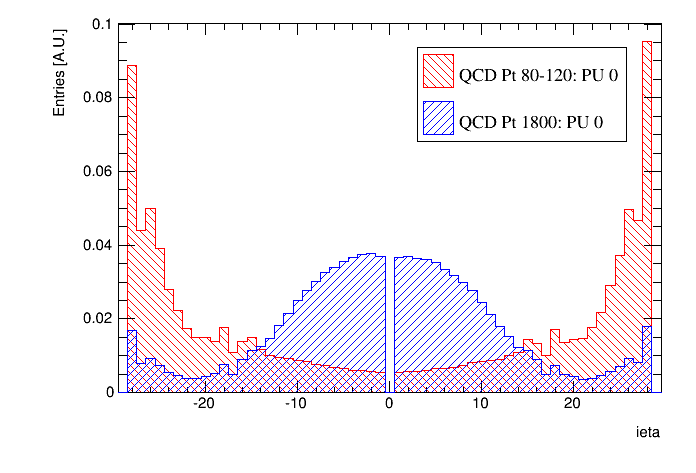
\includegraphics[width=0.8\textwidth]{fig/ieta_comparison_scaled.png}
%% Text
\label{sec-2-2-2-2}
\begin{itemize}

\item \texttt{QCD\_Pt-80to120} dataset more focused on HE (good)
\label{sec-2-2-2-2-1}%
\end{itemize} % ends low level
\end{frame}
\subsection{Processing}
\label{sec-2-3}
\begin{frame}
\frametitle{Processing pileup sample}
\label{sec-2-3-1}
\begin{itemize}

\item Need to overlay \texttt{QCD} with \texttt{MinBias}
\label{sec-2-3-1-1}%

\item Use \texttt{MixingModule} in \texttt{CMSSW\_6\_2\_8}
\label{sec-2-3-1-2}%

\item Pileup scenario: \texttt{AVE\_50\_BX\_25ns}
\label{sec-2-3-1-3}%

\item Two stages:
\label{sec-2-3-1-4}%
\begin{itemize}

\item 1) \texttt{DIGI}, \texttt{L1}, \texttt{DIGI2RAW}, \texttt{HLT}
\label{sec-2-3-1-4-1}%

\item 2) \texttt{RAW2DIGI} \texttt{L1Reco} \texttt{RECO}
\label{sec-2-3-1-4-2}%
\end{itemize} % ends low level

\item Stage 1 all done: \href{https://github.com/edmundaberry/HcalReco/blob/master/test/hcalNoise_fromGEN-SIM_toGEN-SIM-RAW_62X_withMixer_cmsDriver.sh}{\alert{cmsDriver}} and \href{https://github.com/edmundaberry/HcalReco/blob/master/test/hcalNoise_fromGEN-SIM_toGEN-SIM-RAW_62X_withMixer_cfg.py}{\alert{python cfg}}
\label{sec-2-3-1-5}%

\item Stage 2 all done: \href{https://github.com/edmundaberry/HcalReco/blob/master/test/hcalNoise_fromGEN-SIM-RAW_62X_cmsDriver.sh}{\alert{cmsDriver}} and \href{https://github.com/edmundaberry/HcalReco/blob/master/test/hcalNoise_fromGEN-SIM-RAW_62X_cfg.py}{\alert{python cfg}}
\label{sec-2-3-1-6}%

\item High PU is \alert{VERY} CPU intensive: 2 minutes/event
\label{sec-2-3-1-7}%
\end{itemize} % ends low level
\end{frame}
\section{Validation results}
\label{sec-3}
\subsection{Single DIGI comparison}
\label{sec-3-1}
\begin{frame}
\frametitle{PU vs. No PU single digi comparison}
\label{sec-3-1-1}
\begin{columns} % Columns
\label{sec-3-1-1-1}
\begin{column}{0.55\textwidth}
%% Figure
\label{sec-3-1-1-1-1}

\centering
single DIGI comparison: HB
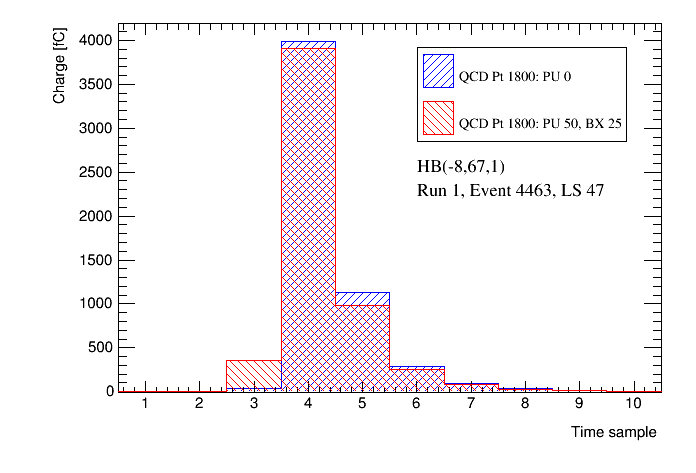
\includegraphics[width=\textwidth]{fig_old/pulse_QCD1800MC_PU_vs_NoPU.png}
\end{column}
\begin{column}{0.55\textwidth}
%% Figure
\label{sec-3-1-1-1-2}

\centering
single DIGI comparison: HE
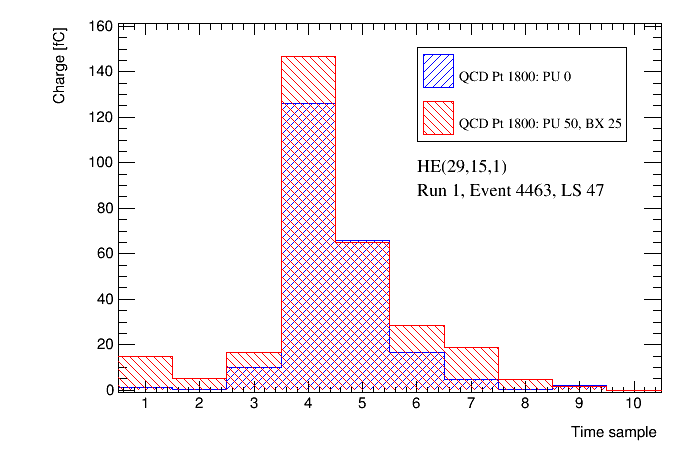
\includegraphics[width=\textwidth]{fig_old/pulse_QCD1800MC_PU_vs_NoPU_HE.png}
\end{column}
\end{columns}
%% Text
\label{sec-3-1-1-2}
\begin{itemize}

\item HE as expected.
\label{sec-3-1-1-2-1}%

\item HB as expected in TS3.  Strangeness in TS4 + TS5.
\label{sec-3-1-1-2-2}%

\item \alert{Focusing on HE}
\label{sec-3-1-1-2-3}%
\end{itemize} % ends low level
\end{frame}
\subsection{Fitting and sanity-checking function on low-PU sample}
\label{sec-3-2}
\begin{frame}
\frametitle{Fits}
\label{sec-3-2-1}
\begin{itemize}

\item Fits have been improved! Better agreement now.
\label{sec-3-2-1-1}%

\item Parameters available on \href{https://github.com/edmundaberry/HcalReco/blob/master/analysis/src/fitResults.C}{\alert{GitHub}}
\label{sec-3-2-1-2}%

\item Same functions as Alexandre for a1, a2, a3
\label{sec-3-2-1-3}%
\begin{itemize}

\item 6 polynomials: 1 for each of 6 regions
\label{sec-3-2-1-3-1}%
\end{itemize} % ends low level

\item For a\_1, this function works better on MC:\\
\label{sec-3-2-1-4}%
\centering
\begin{tabular}{cl}
if $x < [6]$: & $f(x) = [0] \cdot \text{Exp}([1] + [2] \cdot x) + [3] + [4] \cdot x$ \\
if $x > [6]$: & $f(x) = [5] \cdot ( x - [6] ) + c $\\
\end{tabular}

\item $c$ is chosen to ensure continuity of $f(x)$ at $[6]$
\label{sec-3-2-1-5}%
\end{itemize} % ends low level
\end{frame}
\begin{frame}
\frametitle{Function fitting on zero pileup sample: a\_1}
\label{sec-3-2-2}
\begin{columns} % Columns
\label{sec-3-2-2-1}
\begin{column}{0.55\textwidth}
%% Linear
\label{sec-3-2-2-1-1}

\centering
Fit of a\_1 in HB (lin)
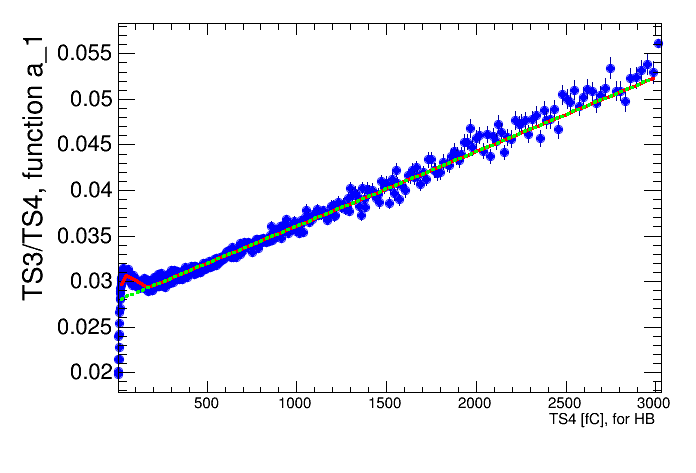
\includegraphics[width=\textwidth]{fig/a0_ring0_lin.png}
\end{column}
\begin{column}{0.55\textwidth}
%% Log
\label{sec-3-2-2-1-2}

\centering
Fit of a\_1 in HB (log)
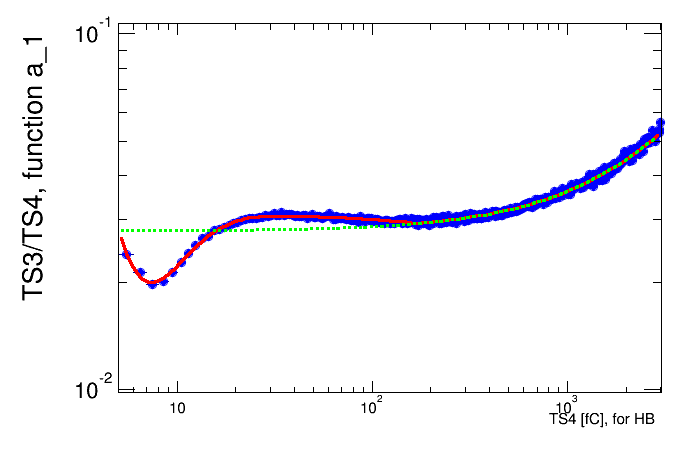
\includegraphics[width=\textwidth]{fig/a0_ring0_log.png}
\end{column}
\end{columns}
%% Text
\label{sec-3-2-2-2}
\begin{itemize}

\item Fit done on zero pileup sample: \alert{use only green line}
\label{sec-3-2-2-2-1}%

\item Fits now extend to TS4 = \alert{3000 fC}
\label{sec-3-2-2-2-2}%

\item Parameters available on \href{https://github.com/edmundaberry/HcalReco/blob/master/analysis/src/fitResults.C}{\alert{GitHub}}
\label{sec-3-2-2-2-3}%
\end{itemize} % ends low level
\end{frame}
\begin{frame}
\frametitle{Function validation on zero pileup sample: a\_1 2D}
\label{sec-3-2-3}
\begin{columns} % Columns
\label{sec-3-2-3-1}
\begin{column}{0.55\textwidth}
%% Full
\label{sec-3-2-3-1-1}

\centering
Validation of a\_1 in HB \\ (TS4 > 0 fC)
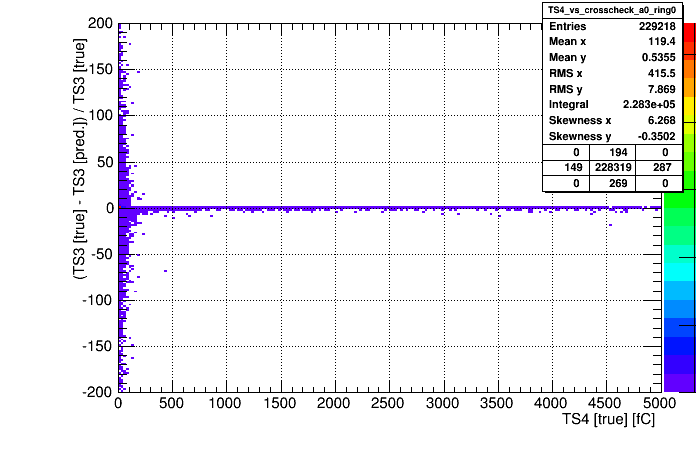
\includegraphics[width=0.8\textwidth]{fig/crosscheck_a0_0.png}
\end{column}
\begin{column}{0.55\textwidth}
%% TS4 > 500 fC
\label{sec-3-2-3-1-2}

\centering
Validation of a\_1 in HB \\ (TS4 > 500 fC)
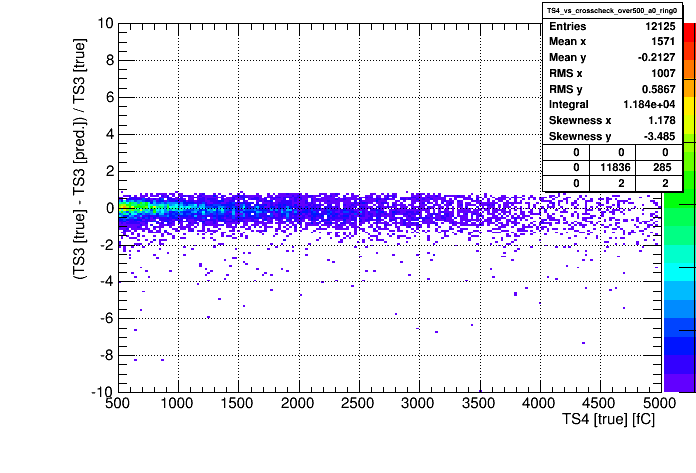
\includegraphics[width=0.8\textwidth]{fig/crosscheck_over500_a0_0.png}
\end{column}
\end{columns}
%% Text
\label{sec-3-2-3-2}
\begin{itemize}

\item Done on zero pileup sample
\label{sec-3-2-3-2-1}%

\item $y$-axis: (TS3 true - TS3 pred.) / TS3 true
\label{sec-3-2-3-2-2}%

\item $x$-axis: TS4 true
\label{sec-3-2-3-2-3}%

\item Spread all at low energy
\label{sec-3-2-3-2-4}%
\end{itemize} % ends low level
\end{frame}
\begin{frame}
\frametitle{Function validation on zero pileup sample: a\_1 1D}
\label{sec-3-2-4}
\begin{columns} % Columns
\label{sec-3-2-4-1}
\begin{column}{0.55\textwidth}
%% TS4 < 500 fC
\label{sec-3-2-4-1-1}

\centering
Validation of a\_1 in HB \\ (TS4 < 50 fC)
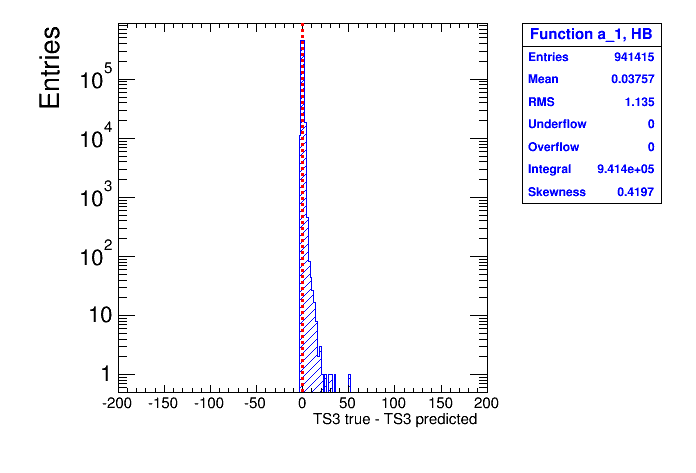
\includegraphics[width=\textwidth]{fig/crosscheck_1D_sample80to120_a0_under50_ring0.png}
\end{column}
\begin{column}{0.55\textwidth}
%% TS4 > 500 fC
\label{sec-3-2-4-1-2}

\centering
Validation of a\_1 in HB \\ (TS4 > 50 fC)
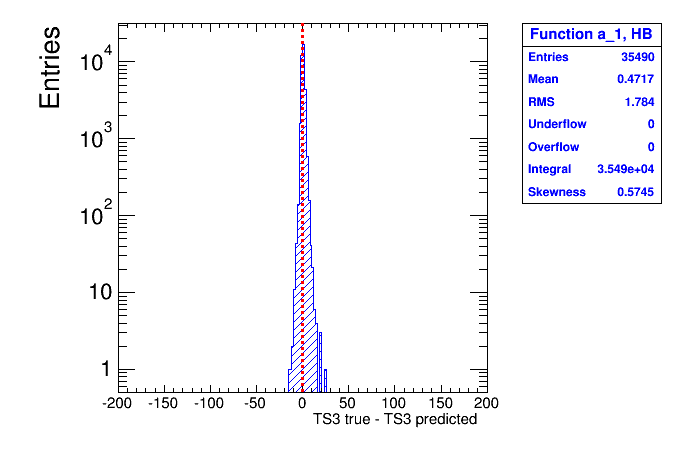
\includegraphics[width=\textwidth]{fig/crosscheck_1D_sample80to120_a0_over50_ring0.png}
\end{column}
\end{columns}
%% Text
\label{sec-3-2-4-2}
\begin{itemize}

\item Done on high pileup, \alert{QCD80to120} sample
\label{sec-3-2-4-2-1}%

\item $x$-axis: TS3 true - TS3 predicted
\label{sec-3-2-4-2-2}%
\end{itemize} % ends low level
\end{frame}
\begin{frame}
\frametitle{Function validation on zero pileup sample: a\_1 1D}
\label{sec-3-2-5}
\begin{columns} % Columns
\label{sec-3-2-5-1}
\begin{column}{0.55\textwidth}
%% TS4 < 500 fC
\label{sec-3-2-5-1-1}

\centering
Validation of a\_1 in HB \\ (TS4 < 500 fC)
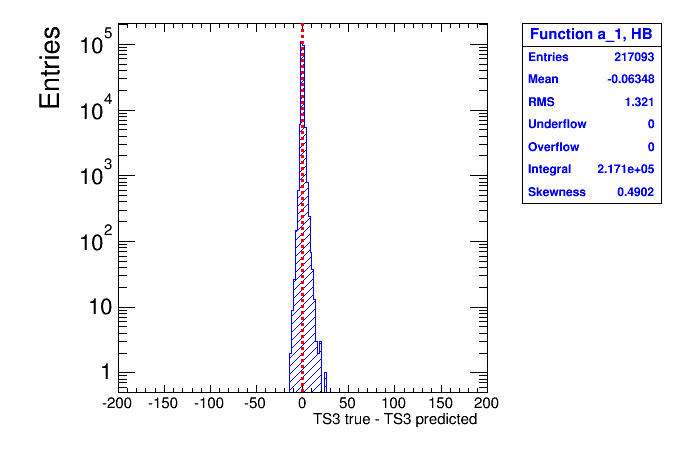
\includegraphics[width=\textwidth]{fig/crosscheck_1D_sample1800_a0_under500_ring0.png}
\end{column}
\begin{column}{0.55\textwidth}
%% TS4 > 500 fC
\label{sec-3-2-5-1-2}

\centering
Validation of a\_1 in HB \\ (TS4 > 500 fC)
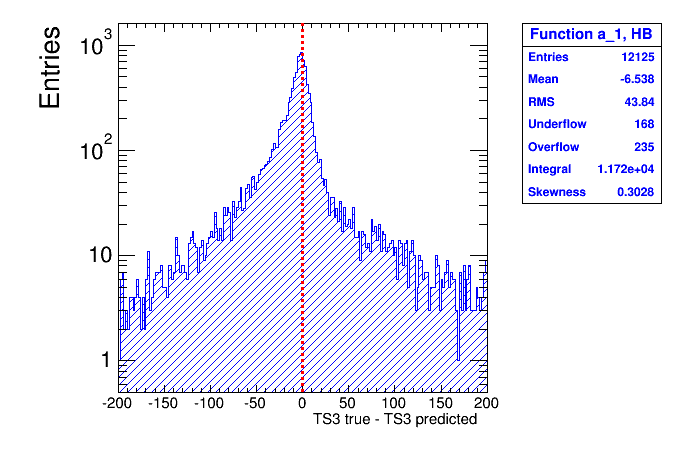
\includegraphics[width=\textwidth]{fig/crosscheck_1D_sample1800_a0_over500_ring0.png}
\end{column}
\end{columns}
%% Text
\label{sec-3-2-5-2}
\begin{itemize}

\item Done on high pileup, \alert{QCD1800} sample
\label{sec-3-2-5-2-1}%

\item $x$-axis: TS3 true - TS3 predicted
\label{sec-3-2-5-2-2}%
\end{itemize} % ends low level
\end{frame}
\begin{frame}
\frametitle{Function fitting on zero pileup sample: a1}
\label{sec-3-2-6}
\begin{columns} % Columns
\label{sec-3-2-6-1}
\begin{column}{0.55\textwidth}
%% Linear
\label{sec-3-2-6-1-1}

\centering
Fit of a1 in HB (lin)
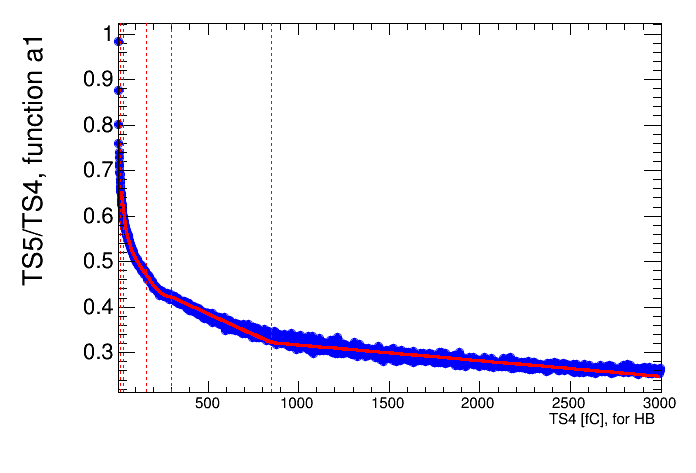
\includegraphics[width=\textwidth]{fig/a1_ring0_lin.png}
\end{column}
\begin{column}{0.55\textwidth}
%% Log
\label{sec-3-2-6-1-2}

\centering
Fit of a1 in HB (log)
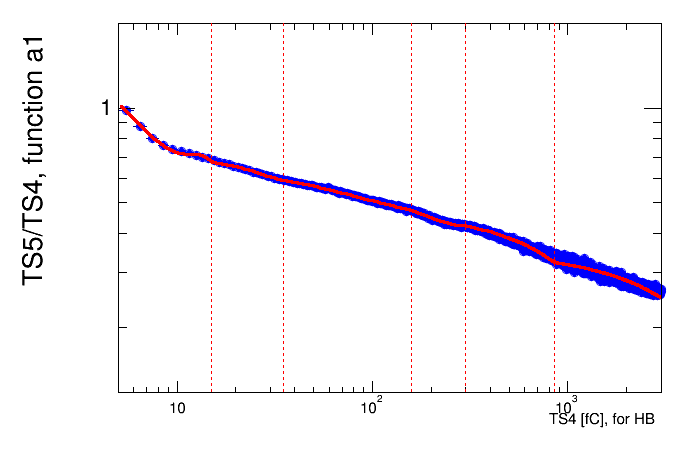
\includegraphics[width=\textwidth]{fig/a1_ring0_log.png}
\end{column}
\end{columns}
%% Text
\label{sec-3-2-6-2}
\begin{itemize}

\item Fit done on zero pileup sample
\label{sec-3-2-6-2-1}%

\item Red lines correspond to fit ranges (Alexandre's functions)
\label{sec-3-2-6-2-2}%

\item Parameters available on \href{https://github.com/edmundaberry/HcalReco/blob/master/analysis/src/fitResults.C}{\alert{GitHub}}
\label{sec-3-2-6-2-3}%
\end{itemize} % ends low level
\end{frame}
\begin{frame}
\frametitle{Function validation on zero pileup sample: a1 2D}
\label{sec-3-2-7}
\begin{columns} % Columns
\label{sec-3-2-7-1}
\begin{column}{0.55\textwidth}
%% Full
\label{sec-3-2-7-1-1}

\centering
Validation of a1 in HB \\ (TS4 > 0 fC)
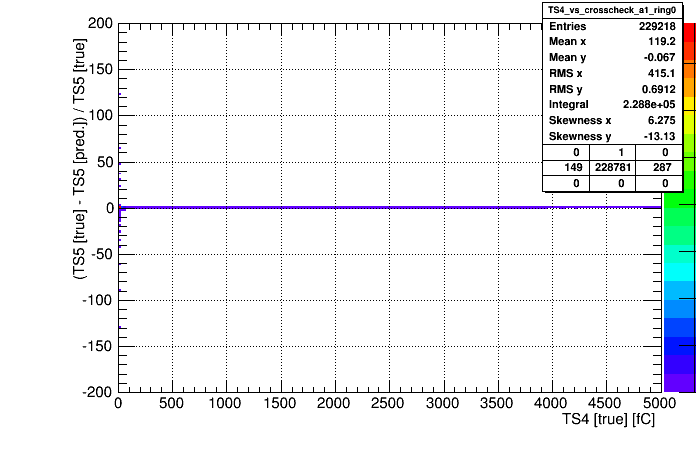
\includegraphics[width=0.8\textwidth]{fig/crosscheck_a1_0.png}
\end{column}
\begin{column}{0.55\textwidth}
%% TS4 > 500 fC
\label{sec-3-2-7-1-2}

\centering
Validation of a1 in HB \\ (TS4 > 500 fC)
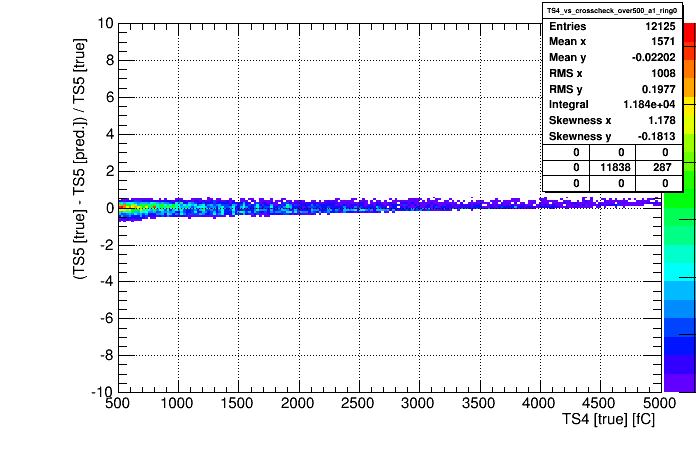
\includegraphics[width=0.8\textwidth]{fig/crosscheck_over500_a1_0.png}
\end{column}
\end{columns}
%% Text
\label{sec-3-2-7-2}
\begin{itemize}

\item Done on zero pileup sample
\label{sec-3-2-7-2-1}%

\item $y$-axis: (TS5 true - TS5 pred.) / TS5 true
\label{sec-3-2-7-2-2}%

\item $x$-axis: TS4 true
\label{sec-3-2-7-2-3}%

\item Better performance than a\_1
\label{sec-3-2-7-2-4}%
\end{itemize} % ends low level
\end{frame}
\begin{frame}
\frametitle{Function validation on zero pileup sample: a1 1D}
\label{sec-3-2-8}
\begin{columns} % Columns
\label{sec-3-2-8-1}
\begin{column}{0.55\textwidth}
%% TS4 < 500 fC
\label{sec-3-2-8-1-1}

\centering
Validation of a1 in HB \\ (TS4 < 50 fC)
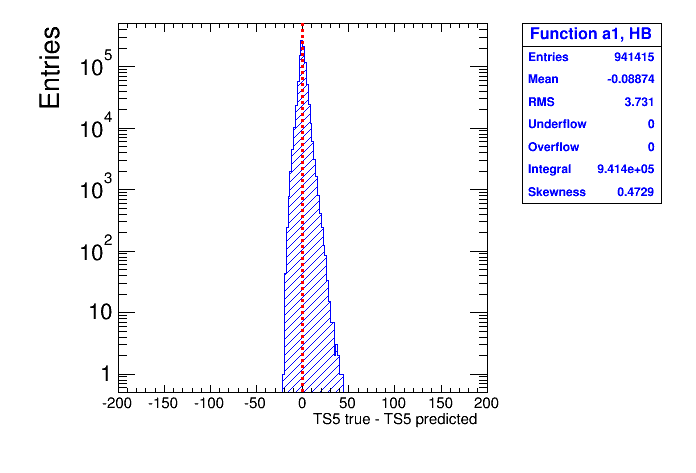
\includegraphics[width=\textwidth]{fig/crosscheck_1D_sample80to120_a1_under50_ring0.png}
\end{column}
\begin{column}{0.55\textwidth}
%% TS4 > 500 fC
\label{sec-3-2-8-1-2}

\centering
Validation of a1 in HB \\ (TS4 > 50 fC)
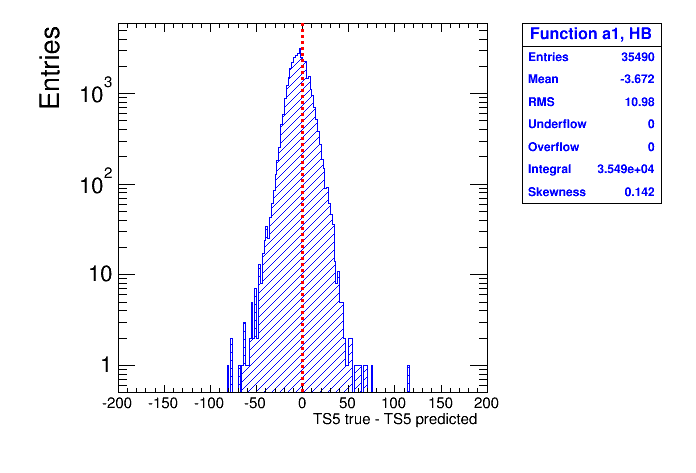
\includegraphics[width=\textwidth]{fig/crosscheck_1D_sample80to120_a1_over50_ring0.png}
\end{column}
\end{columns}
%% Text
\label{sec-3-2-8-2}
\begin{itemize}

\item Done on high pileup, \alert{QCD80to120} sample
\label{sec-3-2-8-2-1}%

\item $x$-axis: TS5 true - TS5 predicted
\label{sec-3-2-8-2-2}%
\end{itemize} % ends low level
\end{frame}
\begin{frame}
\frametitle{Function validation on zero pileup sample: a1 1D}
\label{sec-3-2-9}
\begin{columns} % Columns
\label{sec-3-2-9-1}
\begin{column}{0.55\textwidth}
%% TS4 < 500 fC
\label{sec-3-2-9-1-1}

\centering
Validation of a1 in HB \\ (TS4 < 500 fC)
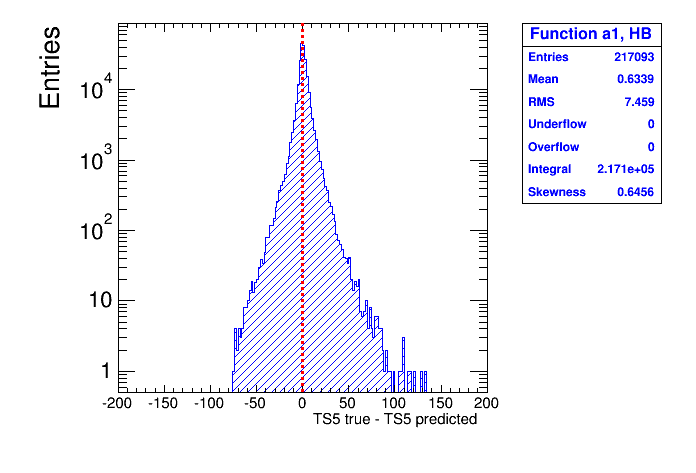
\includegraphics[width=\textwidth]{fig/crosscheck_1D_sample1800_a1_under500_ring0.png}
\end{column}
\begin{column}{0.55\textwidth}
%% TS4 > 500 fC
\label{sec-3-2-9-1-2}

\centering
Validation of a1 in HB \\ (TS4 > 500 fC)
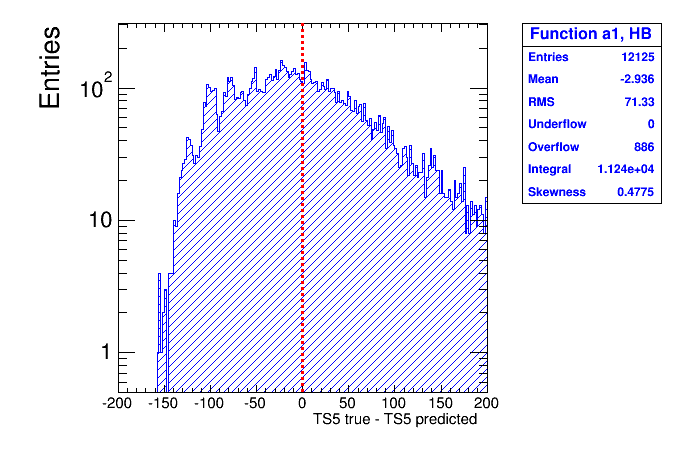
\includegraphics[width=\textwidth]{fig/crosscheck_1D_sample1800_a1_over500_ring0.png}
\end{column}
\end{columns}
%% Text
\label{sec-3-2-9-2}
\begin{itemize}

\item Done on high pileup, \alert{QCD1800} sample
\label{sec-3-2-9-2-1}%

\item $x$-axis: TS5 true - TS5 predicted
\label{sec-3-2-9-2-2}%
\end{itemize} % ends low level
\end{frame}
\begin{frame}
\frametitle{Function fitting on zero pileup sample: a2}
\label{sec-3-2-10}
\begin{columns} % Columns
\label{sec-3-2-10-1}
\begin{column}{0.55\textwidth}
%% Linear
\label{sec-3-2-10-1-1}

\centering
Fit of a2 in HB (lin)
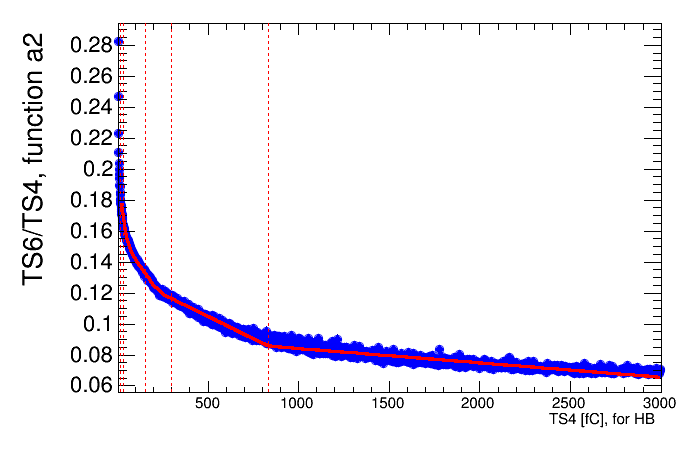
\includegraphics[width=\textwidth]{fig/a2_ring0_lin.png}
\end{column}
\begin{column}{0.55\textwidth}
%% Log
\label{sec-3-2-10-1-2}

\centering
Fit of a2 in HB (log)
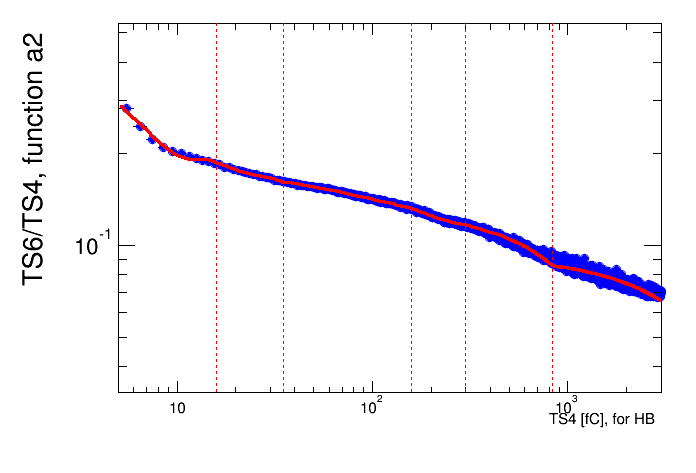
\includegraphics[width=\textwidth]{fig/a2_ring0_log.png}
\end{column}
\end{columns}
%% Text
\label{sec-3-2-10-2}
\begin{itemize}

\item Fit done on zero pileup sample
\label{sec-3-2-10-2-1}%

\item Red lines correspond to fit ranges (Alexandre's functions)
\label{sec-3-2-10-2-2}%

\item Parameters available on \href{https://github.com/edmundaberry/HcalReco/blob/master/analysis/src/fitResults.C}{\alert{GitHub}}
\label{sec-3-2-10-2-3}%
\end{itemize} % ends low level
\end{frame}
\begin{frame}
\frametitle{Function validation on zero pileup sample: a2 2D}
\label{sec-3-2-11}
\begin{columns} % Columns
\label{sec-3-2-11-1}
\begin{column}{0.55\textwidth}
%% Full
\label{sec-3-2-11-1-1}

\centering
Validation of a2 in HB \\ (TS4 > 0 fC)
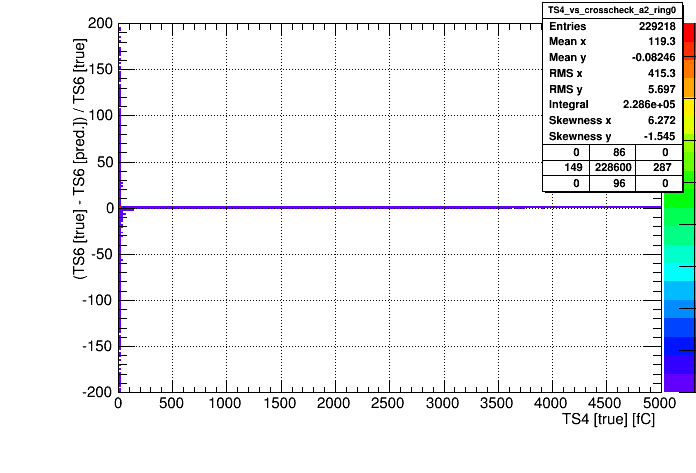
\includegraphics[width=0.8\textwidth]{fig/crosscheck_a2_0.png}
\end{column}
\begin{column}{0.55\textwidth}
%% TS4 > 500 fC
\label{sec-3-2-11-1-2}

\centering
Validation of a2 in HB \\ (TS4 > 500 fC)
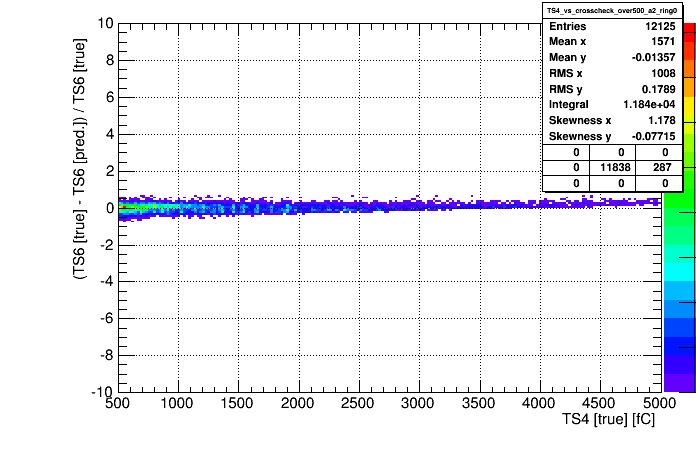
\includegraphics[width=0.8\textwidth]{fig/crosscheck_over500_a2_0.png}
\end{column}
\end{columns}
%% Text
\label{sec-3-2-11-2}
\begin{itemize}

\item Done on zero pileup sample
\label{sec-3-2-11-2-1}%

\item $y$-axis: (TS6 true - TS6 pred.) / TS6 true
\label{sec-3-2-11-2-2}%

\item $x$-axis: TS4 true
\label{sec-3-2-11-2-3}%

\item Better performance than a\_1
\label{sec-3-2-11-2-4}%
\end{itemize} % ends low level
\end{frame}
\begin{frame}
\frametitle{Function validation on zero pileup sample: a2 1D}
\label{sec-3-2-12}
\begin{columns} % Columns
\label{sec-3-2-12-1}
\begin{column}{0.55\textwidth}
%% TS4 < 500 fC
\label{sec-3-2-12-1-1}

\centering
Validation of a2 in HB \\ (TS4 < 50 fC)
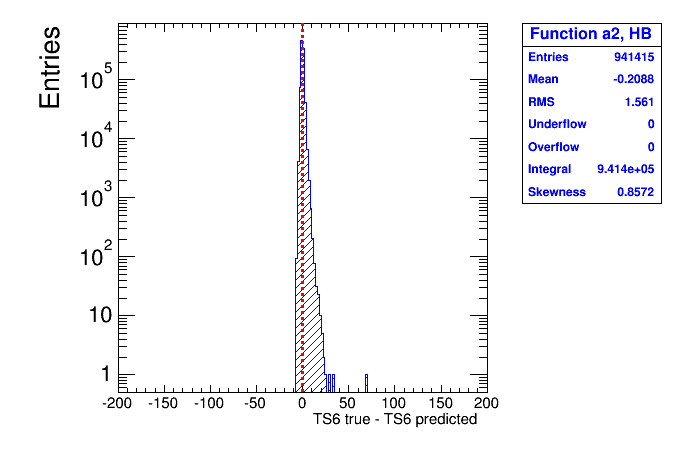
\includegraphics[width=\textwidth]{fig/crosscheck_1D_sample80to120_a2_under50_ring0.png}
\end{column}
\begin{column}{0.55\textwidth}
%% TS4 > 500 fC
\label{sec-3-2-12-1-2}

\centering
Validation of a2 in HB \\ (TS4 > 50 fC)
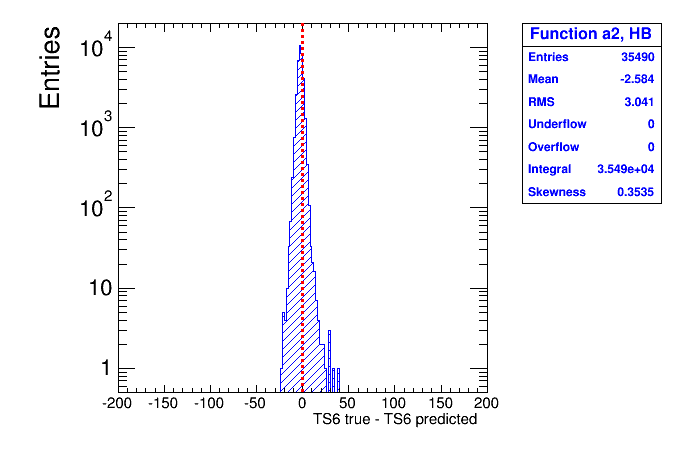
\includegraphics[width=\textwidth]{fig/crosscheck_1D_sample80to120_a2_over50_ring0.png}
\end{column}
\end{columns}
%% Text
\label{sec-3-2-12-2}
\begin{itemize}

\item Done on high pileup, \alert{QCD80to120} sample
\label{sec-3-2-12-2-1}%

\item $x$-axis: TS6 true - TS6 predicted
\label{sec-3-2-12-2-2}%
\end{itemize} % ends low level
\end{frame}
\begin{frame}
\frametitle{Function validation on zero pileup sample: a2 1D}
\label{sec-3-2-13}
\begin{columns} % Columns
\label{sec-3-2-13-1}
\begin{column}{0.55\textwidth}
%% TS4 < 500 fC
\label{sec-3-2-13-1-1}

\centering
Validation of a2 in HB \\ (TS4 < 500 fC)
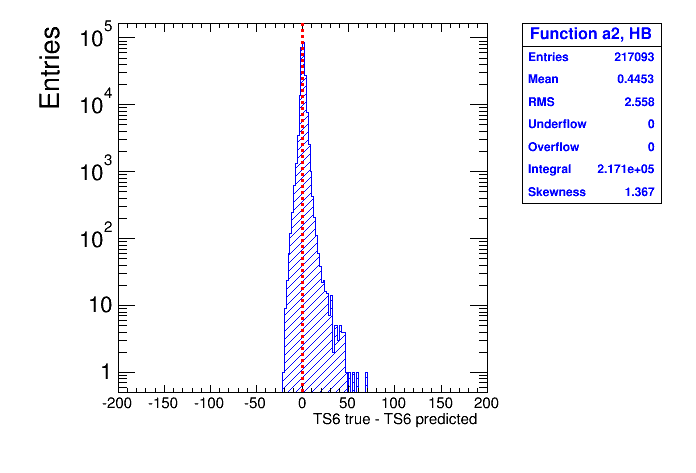
\includegraphics[width=\textwidth]{fig/crosscheck_1D_sample1800_a2_under500_ring0.png}
\end{column}
\begin{column}{0.55\textwidth}
%% TS4 > 500 fC
\label{sec-3-2-13-1-2}

\centering
Validation of a2 in HB \\ (TS4 > 500 fC)
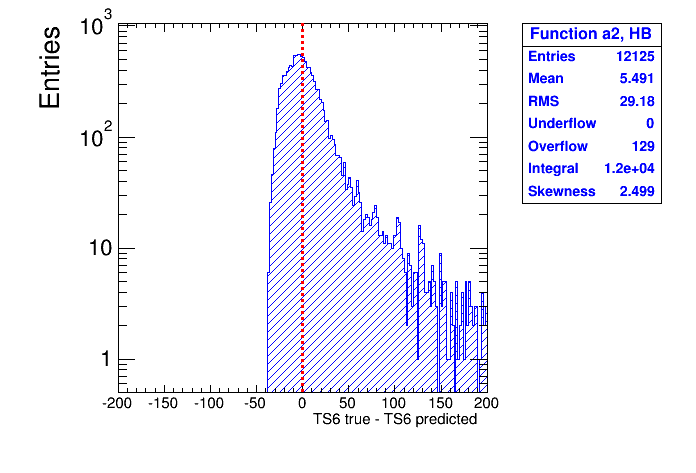
\includegraphics[width=\textwidth]{fig/crosscheck_1D_sample1800_a2_over500_ring0.png}
\end{column}
\end{columns}
%% Text
\label{sec-3-2-13-2}
\begin{itemize}

\item Done on high pileup, \alert{QCD1800} sample
\label{sec-3-2-13-2-1}%

\item $x$-axis: TS6 true - TS6 predicted
\label{sec-3-2-13-2-2}%
\end{itemize} % ends low level
\end{frame}
\begin{frame}
\frametitle{Function fitting on zero pileup sample: a3 2D}
\label{sec-3-2-14}
\begin{columns} % Columns
\label{sec-3-2-14-1}
\begin{column}{0.55\textwidth}
%% Linear
\label{sec-3-2-14-1-1}

\centering
Fit of a3 in HB (lin)
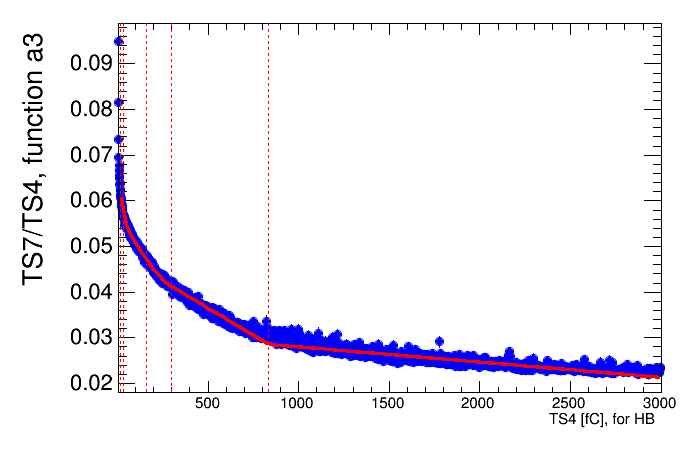
\includegraphics[width=\textwidth]{fig/a3_ring0_lin.png}
\end{column}
\begin{column}{0.55\textwidth}
%% Log
\label{sec-3-2-14-1-2}

\centering
Fit of a3 in HB (log)
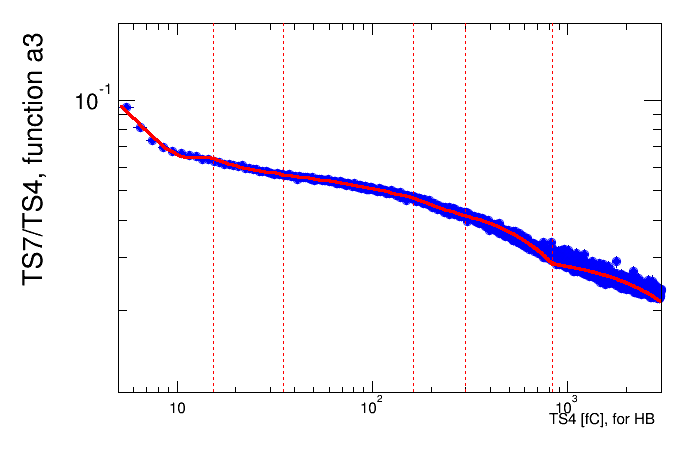
\includegraphics[width=\textwidth]{fig/a3_ring0_log.png}
\end{column}
\end{columns}
%% Text
\label{sec-3-2-14-2}
\begin{itemize}

\item Fit done on zero pileup sample
\label{sec-3-2-14-2-1}%

\item Red lines correspond to fit ranges (Alexandre's functions)
\label{sec-3-2-14-2-2}%

\item Parameters available on \href{https://github.com/edmundaberry/HcalReco/blob/master/analysis/src/fitResults.C}{\alert{GitHub}}
\label{sec-3-2-14-2-3}%
\end{itemize} % ends low level
\end{frame}
\begin{frame}
\frametitle{Function validation on zero pileup sample: a3 1D}
\label{sec-3-2-15}
\begin{columns} % Columns
\label{sec-3-2-15-1}
\begin{column}{0.55\textwidth}
%% TS4 < 500 fC
\label{sec-3-2-15-1-1}

\centering
Validation of a3 in HB \\ (TS4 < 50 fC)
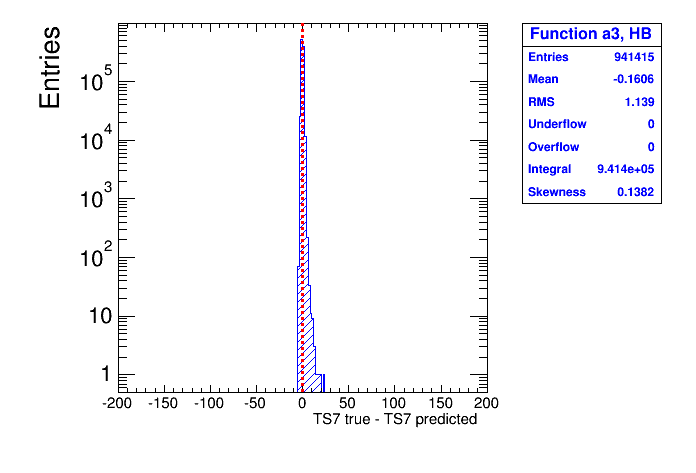
\includegraphics[width=\textwidth]{fig/crosscheck_1D_sample80to120_a3_under50_ring0.png}
\end{column}
\begin{column}{0.55\textwidth}
%% TS4 > 500 fC
\label{sec-3-2-15-1-2}

\centering
Validation of a3 in HB \\ (TS4 > 50 fC)
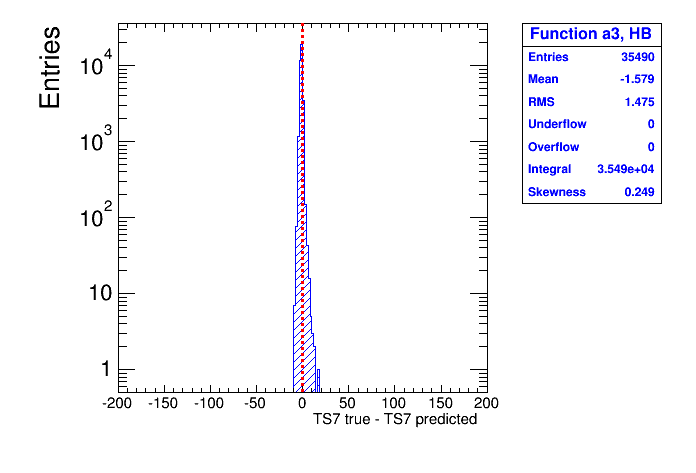
\includegraphics[width=\textwidth]{fig/crosscheck_1D_sample80to120_a3_over50_ring0.png}
\end{column}
\end{columns}
%% Text
\label{sec-3-2-15-2}
\begin{itemize}

\item Done on high pileup, \alert{QCD80to120} sample
\label{sec-3-2-15-2-1}%

\item $x$-axis: TS7 true - TS7 predicted
\label{sec-3-2-15-2-2}%
\end{itemize} % ends low level
\end{frame}
\begin{frame}
\frametitle{Function validation on zero pileup sample: a3 1D}
\label{sec-3-2-16}
\begin{columns} % Columns
\label{sec-3-2-16-1}
\begin{column}{0.55\textwidth}
%% TS4 < 500 fC
\label{sec-3-2-16-1-1}

\centering
Validation of a3 in HB \\ (TS4 < 500 fC)
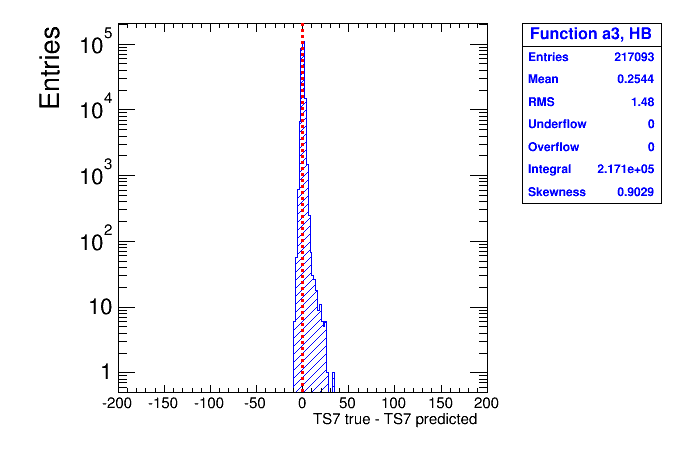
\includegraphics[width=\textwidth]{fig/crosscheck_1D_sample1800_a3_under500_ring0.png}
\end{column}
\begin{column}{0.55\textwidth}
%% TS4 > 500 fC
\label{sec-3-2-16-1-2}

\centering
Validation of a3 in HB \\ (TS4 > 500 fC)
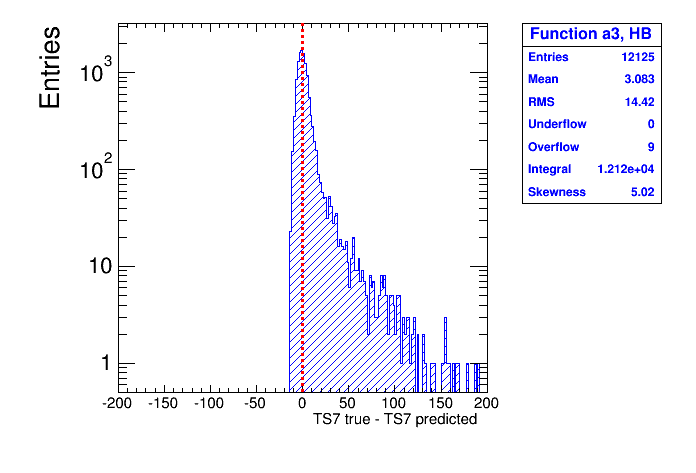
\includegraphics[width=\textwidth]{fig/crosscheck_1D_sample1800_a3_over500_ring0.png}
\end{column}
\end{columns}
%% Text
\label{sec-3-2-16-2}
\begin{itemize}

\item Done on high pileup, \alert{QCD1800} sample
\label{sec-3-2-16-2-1}%

\item $x$-axis: TS7 true - TS7 predicted
\label{sec-3-2-16-2-2}%

\end{itemize} % ends low level
\end{frame}
\subsection{Validating on high-PU sample}
\label{sec-3-3}
\begin{frame}
\frametitle{Results in HB: 2D}
\label{sec-3-3-1}
\begin{columns} % Columns
\label{sec-3-3-1-1}
\begin{column}{0.55\textwidth}
%% Figure
\label{sec-3-3-1-1-1}

\centering
No correction applied
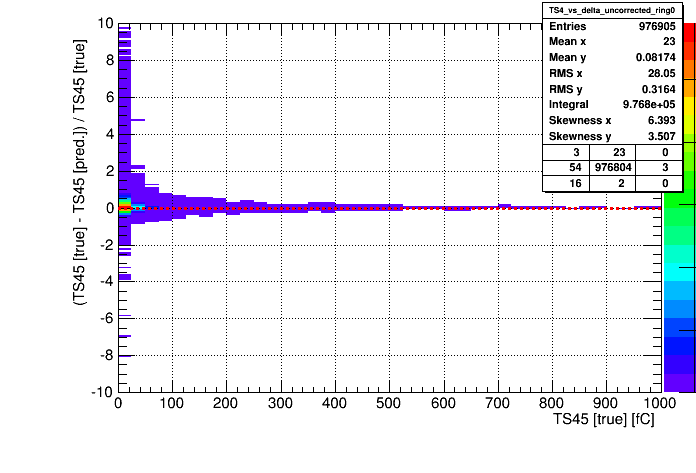
\includegraphics[width=0.8\textwidth]{fig/delta_uncorrected_QCD80to120_ring_0.png}
\end{column}
\begin{column}{0.55\textwidth}
%% Figure
\label{sec-3-3-1-1-2}

\centering
With correction applied
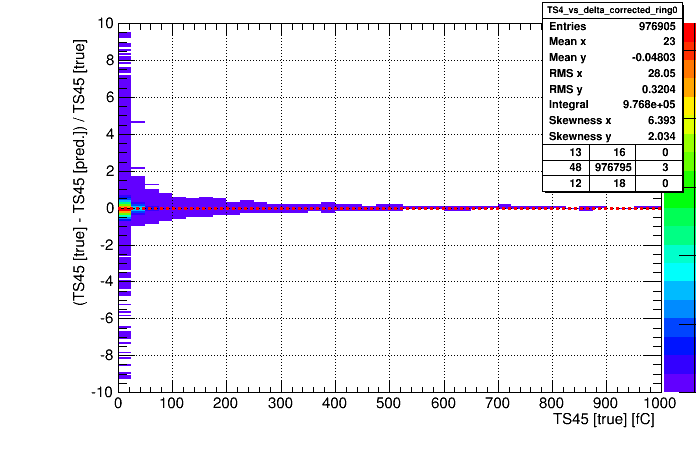
\includegraphics[width=0.8\textwidth]{fig/delta_corrected_QCD80to120_ring_0.png}
\end{column}
\end{columns}
%% Text
\label{sec-3-3-1-2}
\begin{itemize}

\item Done on high pileup, \alert{QCD80to120} sample
\label{sec-3-3-1-2-1}%

\item $y$-axis: (TS45 true - TS45 pred.) / TS45 true
\label{sec-3-3-1-2-2}%

\item $x$-axis: TS45 true
\label{sec-3-3-1-2-3}%
\end{itemize} % ends low level
\end{frame}
\begin{frame}
\frametitle{Results in HB: 2D}
\label{sec-3-3-2}
\begin{columns} % Columns
\label{sec-3-3-2-1}
\begin{column}{0.55\textwidth}
%% Figure
\label{sec-3-3-2-1-1}

\centering
No correction applied
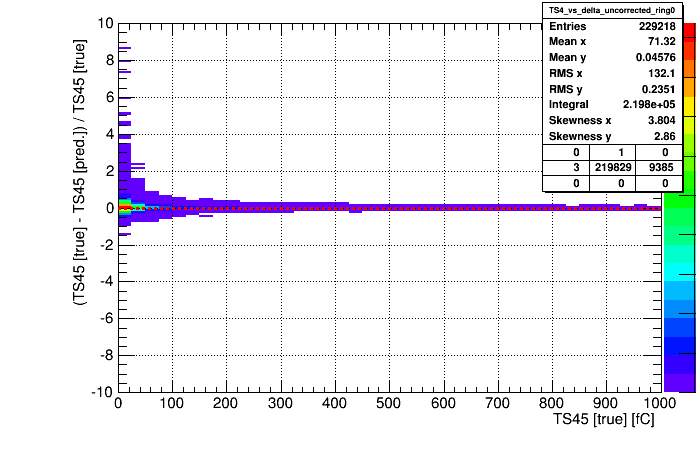
\includegraphics[width=0.8\textwidth]{fig/delta_uncorrected_QCD1800_ring_0.png}
\end{column}
\begin{column}{0.55\textwidth}
%% Figure
\label{sec-3-3-2-1-2}

\centering
With correction applied
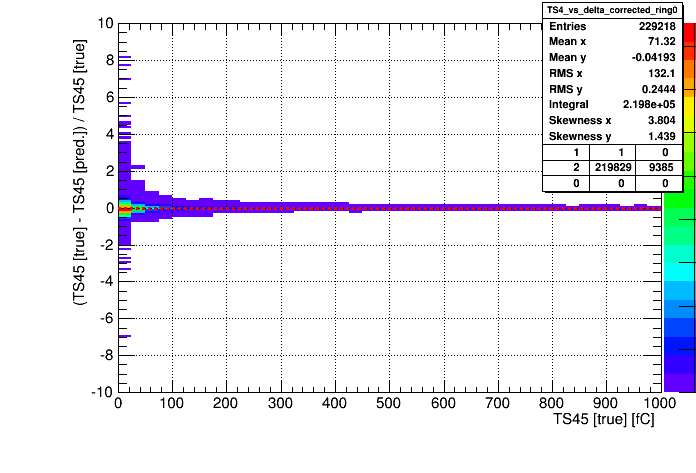
\includegraphics[width=0.8\textwidth]{fig/delta_corrected_QCD1800_ring_0.png}
\end{column}
\end{columns}
%% Text
\label{sec-3-3-2-2}
\begin{itemize}

\item Done on high pileup, \alert{QCD1800} sample
\label{sec-3-3-2-2-1}%

\item $y$-axis: (TS45 true - TS45 pred.) / TS45 true
\label{sec-3-3-2-2-2}%

\item $x$-axis: TS45 true
\label{sec-3-3-2-2-3}%
\end{itemize} % ends low level
\end{frame}
\begin{frame}
\frametitle{Results in HB: 1D}
\label{sec-3-3-3}
\begin{columns} % Columns
\label{sec-3-3-3-1}
\begin{column}{0.55\textwidth}
%% Figure
\label{sec-3-3-3-1-1}

\centering
TS4 < 50 fC
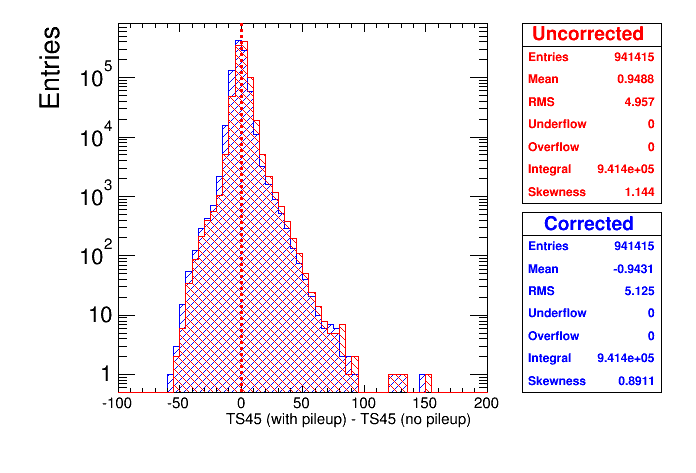
\includegraphics[width=\textwidth]{fig/correction_comparison_1D_sample80to120_under50_ring0.png}
\end{column}
\begin{column}{0.55\textwidth}
%% Figure
\label{sec-3-3-3-1-2}

\centering
TS4 > 50 fC
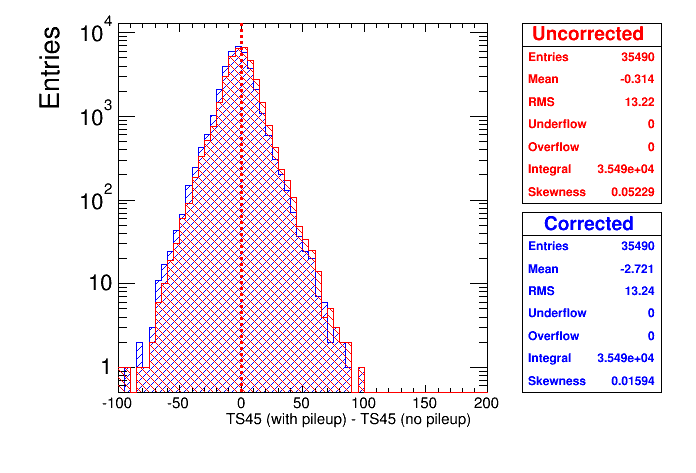
\includegraphics[width=\textwidth]{fig/correction_comparison_1D_sample80to120_over50_ring0.png}
\end{column}
\end{columns}
%% Text
\label{sec-3-3-3-2}
\begin{itemize}

\item Done on high pileup, \alert{QCD80to120} sample
\label{sec-3-3-3-2-1}%

\item $x$-axis: TS45 true - TS45 pred, $y$-axis: Entries
\label{sec-3-3-3-2-2}%

\item Corrections make little difference in the barrel
\label{sec-3-3-3-2-3}%
\end{itemize} % ends low level
\end{frame}
\begin{frame}
\frametitle{Results in HB: 1D}
\label{sec-3-3-4}
\begin{columns} % Columns
\label{sec-3-3-4-1}
\begin{column}{0.55\textwidth}
%% Figure
\label{sec-3-3-4-1-1}

\centering
TS4 < 500 fC
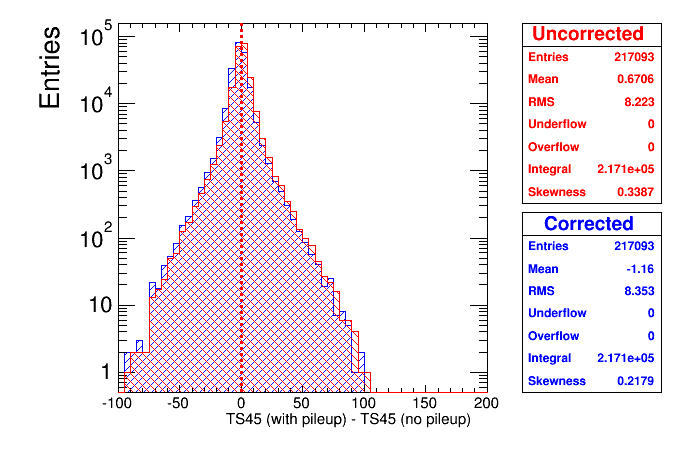
\includegraphics[width=\textwidth]{fig/correction_comparison_1D_sample1800_under500_ring0.png}
\end{column}
\begin{column}{0.55\textwidth}
%% Figure
\label{sec-3-3-4-1-2}

\centering
TS4 > 500 fC
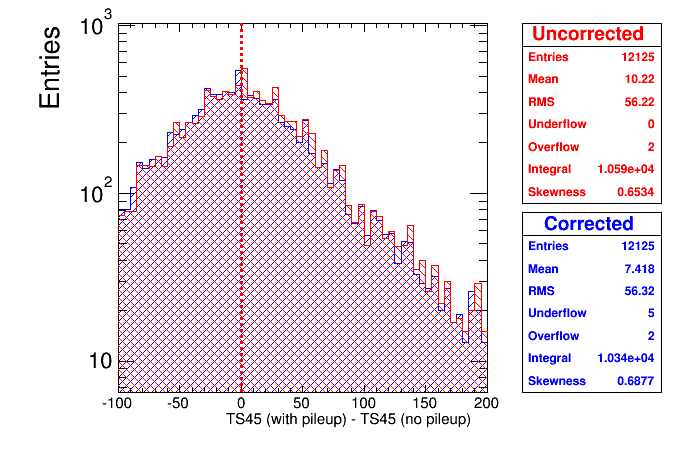
\includegraphics[width=\textwidth]{fig/correction_comparison_1D_sample1800_over500_ring0.png}
\end{column}
\end{columns}
%% Text
\label{sec-3-3-4-2}
\begin{itemize}

\item Done on high pileup, \alert{QCD1800} sample
\label{sec-3-3-4-2-1}%

\item $x$-axis: TS45 true - TS45 pred, $y$-axis: Entries
\label{sec-3-3-4-2-2}%

\item Corrections make little difference in the barrel
\label{sec-3-3-4-2-3}%
\end{itemize} % ends low level
\end{frame}
\begin{frame}
\frametitle{Results in HE 17-20: 2D}
\label{sec-3-3-5}
\begin{columns} % Columns
\label{sec-3-3-5-1}
\begin{column}{0.55\textwidth}
%% Figure
\label{sec-3-3-5-1-1}

\centering
No correction applied
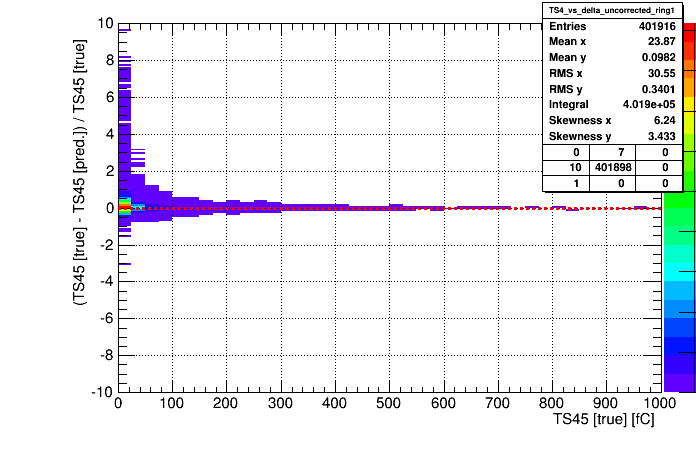
\includegraphics[width=0.8\textwidth]{fig/delta_uncorrected_QCD80to120_ring_1.png}
\end{column}
\begin{column}{0.55\textwidth}
%% Figure
\label{sec-3-3-5-1-2}

\centering
With correction applied
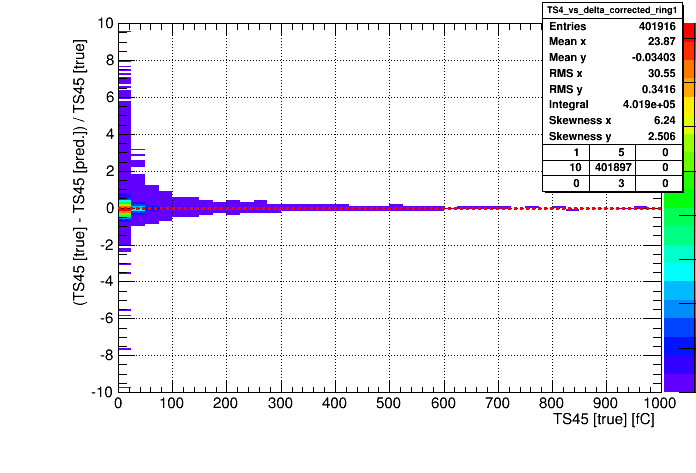
\includegraphics[width=0.8\textwidth]{fig/delta_corrected_QCD80to120_ring_1.png}
\end{column}
\end{columns}
%% Text
\label{sec-3-3-5-2}
\begin{itemize}

\item Done on high pileup, \alert{QCD80to120} sample
\label{sec-3-3-5-2-1}%

\item $y$-axis: (TS45 true - TS45 pred.) / TS45 true
\label{sec-3-3-5-2-2}%

\item $x$-axis: TS45 true
\label{sec-3-3-5-2-3}%

\end{itemize} % ends low level
\end{frame}
\begin{frame}
\frametitle{Results in HE 17-20: 2D}
\label{sec-3-3-6}
\begin{columns} % Columns
\label{sec-3-3-6-1}
\begin{column}{0.55\textwidth}
%% Figure
\label{sec-3-3-6-1-1}

\centering
No correction applied
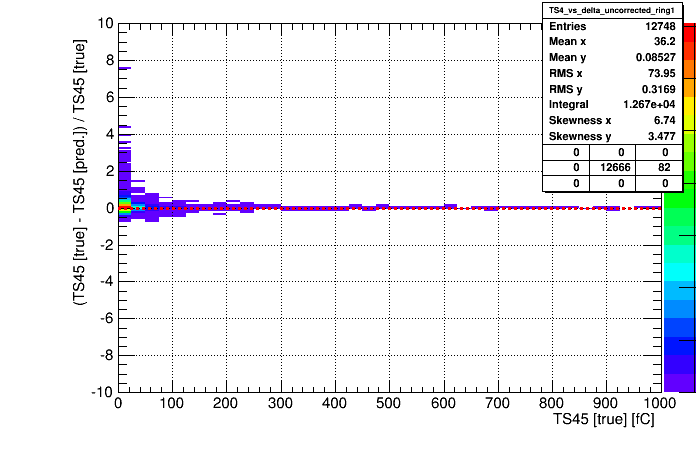
\includegraphics[width=0.8\textwidth]{fig/delta_uncorrected_QCD1800_ring_1.png}
\end{column}
\begin{column}{0.55\textwidth}
%% Figure
\label{sec-3-3-6-1-2}

\centering
With correction applied
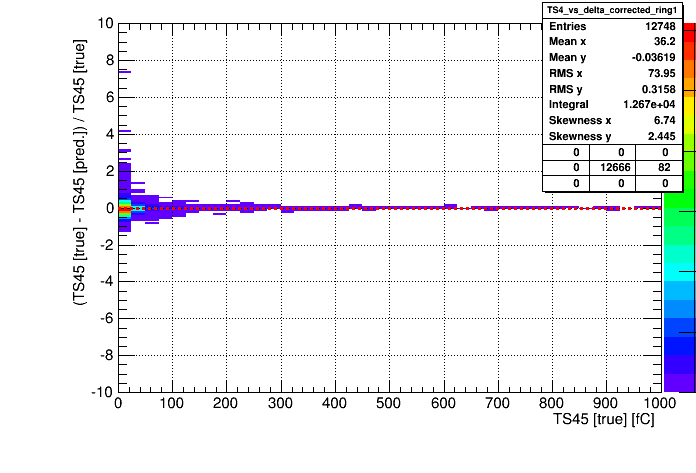
\includegraphics[width=0.8\textwidth]{fig/delta_corrected_QCD1800_ring_1.png}
\end{column}
\end{columns}
%% Text
\label{sec-3-3-6-2}
\begin{itemize}

\item Done on high pileup, \alert{QCD1800} sample
\label{sec-3-3-6-2-1}%

\item $y$-axis: (TS45 true - TS45 pred.) / TS45 true
\label{sec-3-3-6-2-2}%

\item $x$-axis: TS45 true
\label{sec-3-3-6-2-3}%

\end{itemize} % ends low level
\end{frame}
\begin{frame}
\frametitle{Results in HE 17-20: 1D}
\label{sec-3-3-7}
\begin{columns} % Columns
\label{sec-3-3-7-1}
\begin{column}{0.55\textwidth}
%% Figure
\label{sec-3-3-7-1-1}

\centering
TS4 < 50 fC
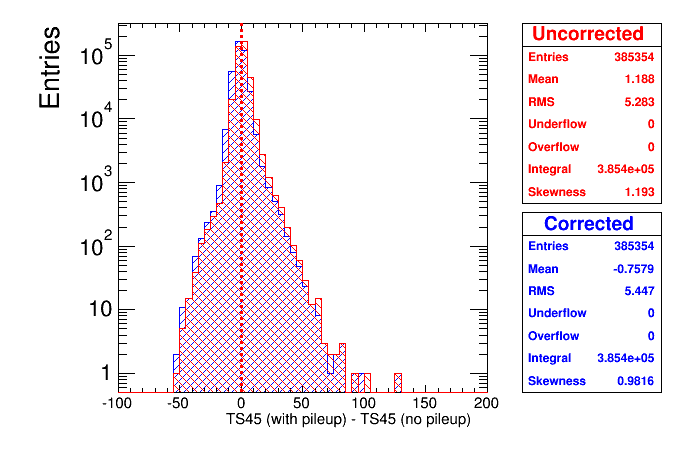
\includegraphics[width=\textwidth]{fig/correction_comparison_1D_sample80to120_under50_ring1.png}
\end{column}
\begin{column}{0.55\textwidth}
%% Figure
\label{sec-3-3-7-1-2}

\centering
TS4 > 50 fC
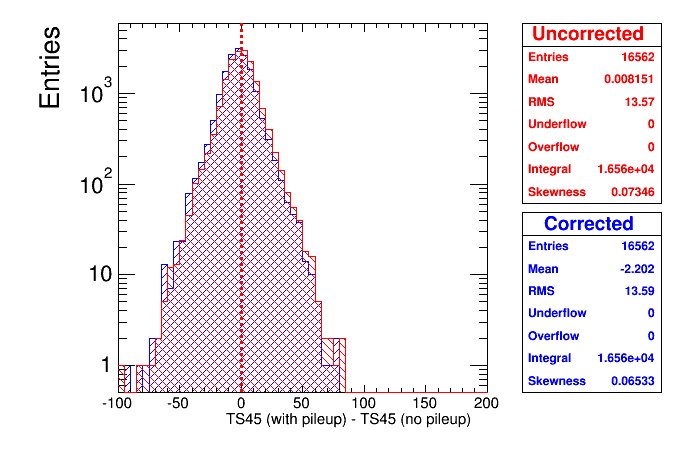
\includegraphics[width=\textwidth]{fig/correction_comparison_1D_sample80to120_over50_ring1.png}
\end{column}
\end{columns}
%% Text
\label{sec-3-3-7-2}
\begin{itemize}

\item Done on high pileup, \alert{QCD80to120} sample
\label{sec-3-3-7-2-1}%

\item $x$-axis: TS45 true - TS45 pred, $y$-axis: Entries
\label{sec-3-3-7-2-2}%

\item Start to see effect of corrections in the low-eta endcap
\label{sec-3-3-7-2-3}%
\end{itemize} % ends low level
\end{frame}
\begin{frame}
\frametitle{Results in HE 17-20: 1D}
\label{sec-3-3-8}
\begin{columns} % Columns
\label{sec-3-3-8-1}
\begin{column}{0.55\textwidth}
%% Figure
\label{sec-3-3-8-1-1}

\centering
TS4 < 500 fC
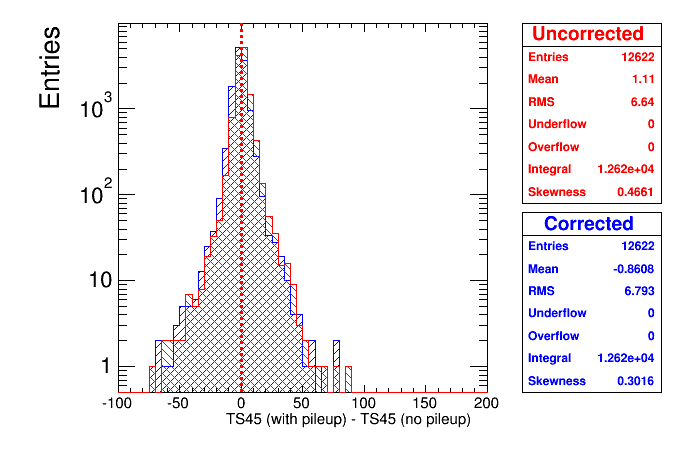
\includegraphics[width=\textwidth]{fig/correction_comparison_1D_sample1800_under500_ring1.png}
\end{column}
\begin{column}{0.55\textwidth}
%% Figure
\label{sec-3-3-8-1-2}

\centering
TS4 > 500 fC
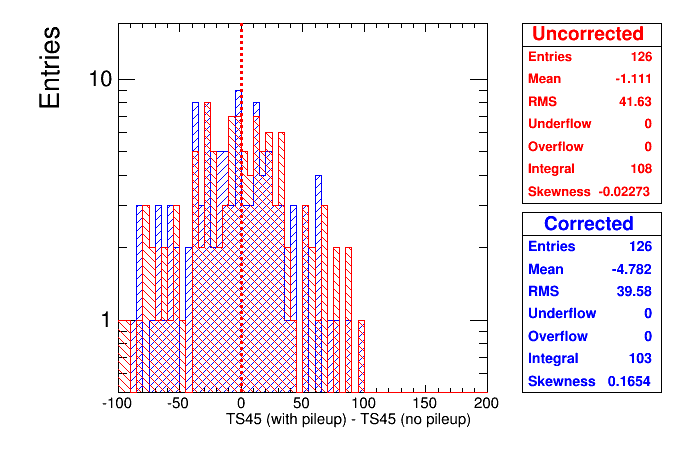
\includegraphics[width=\textwidth]{fig/correction_comparison_1D_sample1800_over500_ring1.png}
\end{column}
\end{columns}
%% Text
\label{sec-3-3-8-2}
\begin{itemize}

\item Done on high pileup, \alert{QCD1800} sample
\label{sec-3-3-8-2-1}%

\item $x$-axis: TS45 true - TS45 pred, $y$-axis: Entries
\label{sec-3-3-8-2-2}%

\item Start to see effect of corrections in the low-eta endcap
\label{sec-3-3-8-2-3}%
\end{itemize} % ends low level
\end{frame}
\begin{frame}
\frametitle{Results in HE 21-23: 2D}
\label{sec-3-3-9}
\begin{columns} % Columns
\label{sec-3-3-9-1}
\begin{column}{0.55\textwidth}
%% Figure
\label{sec-3-3-9-1-1}

\centering
No correction applied
\includegraphics[width=0.8\textwidth]{fig/delta_uncorrected_QCD80to120_ring_2.png}
\end{column}
\begin{column}{0.55\textwidth}
%% Figure
\label{sec-3-3-9-1-2}

\centering
With correction applied
\includegraphics[width=0.8\textwidth]{fig/delta_corrected_QCD80to120_ring_2.png}
\end{column}
\end{columns}
%% Text
\label{sec-3-3-9-2}
\begin{itemize}

\item Done on high pileup, \alert{QCD80to120} sample
\label{sec-3-3-9-2-1}%

\item $y$-axis: (TS45 true - TS45 pred.) / TS45 true
\label{sec-3-3-9-2-2}%

\item $x$-axis: TS45 true
\label{sec-3-3-9-2-3}%

\end{itemize} % ends low level
\end{frame}
\begin{frame}
\frametitle{Results in HE 21-23: 2D}
\label{sec-3-3-10}
\begin{columns} % Columns
\label{sec-3-3-10-1}
\begin{column}{0.55\textwidth}
%% Figure
\label{sec-3-3-10-1-1}

\centering
No correction applied
\includegraphics[width=0.8\textwidth]{fig/delta_uncorrected_QCD1800_ring_2.png}
\end{column}
\begin{column}{0.55\textwidth}
%% Figure
\label{sec-3-3-10-1-2}

\centering
With correction applied
\includegraphics[width=0.8\textwidth]{fig/delta_corrected_QCD1800_ring_2.png}
\end{column}
\end{columns}
%% Text
\label{sec-3-3-10-2}
\begin{itemize}

\item Done on high pileup, \alert{QCD1800} sample
\label{sec-3-3-10-2-1}%

\item $y$-axis: (TS45 true - TS45 pred.) / TS45 true
\label{sec-3-3-10-2-2}%

\item $x$-axis: TS45 true
\label{sec-3-3-10-2-3}%

\end{itemize} % ends low level
\end{frame}
\begin{frame}
\frametitle{Results in HE 21-23: 1D}
\label{sec-3-3-11}
\begin{columns} % Columns
\label{sec-3-3-11-1}
\begin{column}{0.55\textwidth}
%% Figure
\label{sec-3-3-11-1-1}

\centering
TS4 < 50 fC
\includegraphics[width=\textwidth]{fig/correction_comparison_1D_sample80to120_under50_ring2.png}
\end{column}
\begin{column}{0.55\textwidth}
%% Figure
\label{sec-3-3-11-1-2}

\centering
TS4 > 50 fC
\includegraphics[width=\textwidth]{fig/correction_comparison_1D_sample80to120_over50_ring2.png}
\end{column}
\end{columns}
%% Text
\label{sec-3-3-11-2}
\begin{itemize}

\item Done on high pileup, \alert{QCD80to120} sample
\label{sec-3-3-11-2-1}%

\item $x$-axis: TS45 true - TS45 pred, $y$-axis: Entries
\label{sec-3-3-11-2-2}%

\item Start to see effect of corrections in the low-eta endcap
\label{sec-3-3-11-2-3}%
\end{itemize} % ends low level
\end{frame}
\begin{frame}
\frametitle{Results in HE 21-23: 1D}
\label{sec-3-3-12}
\begin{columns} % Columns
\label{sec-3-3-12-1}
\begin{column}{0.55\textwidth}
%% Figure
\label{sec-3-3-12-1-1}

\centering
TS4 < 500 fC
\includegraphics[width=\textwidth]{fig/correction_comparison_1D_sample1800_under500_ring2.png}
\end{column}
\begin{column}{0.55\textwidth}
%% Figure
\label{sec-3-3-12-1-2}

\centering
TS4 > 500 fC
\includegraphics[width=\textwidth]{fig/correction_comparison_1D_sample1800_over500_ring2.png}
\end{column}
\end{columns}
%% Text
\label{sec-3-3-12-2}
\begin{itemize}

\item Done on high pileup, \alert{QCD1800} sample
\label{sec-3-3-12-2-1}%

\item $x$-axis: TS45 true - TS45 pred, $y$-axis: Entries
\label{sec-3-3-12-2-2}%

\item Start to see effect of corrections in the low-eta endcap
\label{sec-3-3-12-2-3}%
\end{itemize} % ends low level
\end{frame}
\begin{frame}
\frametitle{Results in HE 24-25: 2D}
\label{sec-3-3-13}
\begin{columns} % Columns
\label{sec-3-3-13-1}
\begin{column}{0.55\textwidth}
%% Figure
\label{sec-3-3-13-1-1}

\centering
No correction applied
\includegraphics[width=0.8\textwidth]{fig/delta_uncorrected_QCD80to120_ring_3.png}
\end{column}
\begin{column}{0.55\textwidth}
%% Figure
\label{sec-3-3-13-1-2}

\centering
With correction applied
\includegraphics[width=0.8\textwidth]{fig/delta_corrected_QCD80to120_ring_3.png}
\end{column}
\end{columns}
%% Text
\label{sec-3-3-13-2}
\begin{itemize}

\item Done on high pileup, \alert{QCD80to120} sample
\label{sec-3-3-13-2-1}%

\item $y$-axis: (TS45 true - TS45 pred.) / TS45 true
\label{sec-3-3-13-2-2}%

\item $x$-axis: TS45 true
\label{sec-3-3-13-2-3}%

\end{itemize} % ends low level
\end{frame}
\begin{frame}
\frametitle{Results in HE 24-25: 2D}
\label{sec-3-3-14}
\begin{columns} % Columns
\label{sec-3-3-14-1}
\begin{column}{0.55\textwidth}
%% Figure
\label{sec-3-3-14-1-1}

\centering
No correction applied
\includegraphics[width=0.8\textwidth]{fig/delta_uncorrected_QCD1800_ring_3.png}
\end{column}
\begin{column}{0.55\textwidth}
%% Figure
\label{sec-3-3-14-1-2}

\centering
With correction applied
\includegraphics[width=0.8\textwidth]{fig/delta_corrected_QCD1800_ring_3.png}
\end{column}
\end{columns}
%% Text
\label{sec-3-3-14-2}
\begin{itemize}

\item Done on high pileup, \alert{QCD1800} sample
\label{sec-3-3-14-2-1}%

\item $y$-axis: (TS45 true - TS45 pred.) / TS45 true
\label{sec-3-3-14-2-2}%

\item $x$-axis: TS45 true
\label{sec-3-3-14-2-3}%

\end{itemize} % ends low level
\end{frame}
\begin{frame}
\frametitle{Results in HE 24-25: 1D}
\label{sec-3-3-15}
\begin{columns} % Columns
\label{sec-3-3-15-1}
\begin{column}{0.55\textwidth}
%% Figure
\label{sec-3-3-15-1-1}

\centering
TS4 < 50 fC
\includegraphics[width=\textwidth]{fig/correction_comparison_1D_sample80to120_under50_ring3.png}
\end{column}
\begin{column}{0.55\textwidth}
%% Figure
\label{sec-3-3-15-1-2}

\centering
TS4 > 50 fC
\includegraphics[width=\textwidth]{fig/correction_comparison_1D_sample80to120_over50_ring3.png}
\end{column}
\end{columns}
%% Text
\label{sec-3-3-15-2}
\begin{itemize}

\item Done on high pileup, \alert{QCD80to120} sample
\label{sec-3-3-15-2-1}%

\item $x$-axis: TS45 true - TS45 pred, $y$-axis: Entries
\label{sec-3-3-15-2-2}%
\end{itemize} % ends low level
\end{frame}
\begin{frame}
\frametitle{Results in HE 24-25: 1D}
\label{sec-3-3-16}
\begin{columns} % Columns
\label{sec-3-3-16-1}
\begin{column}{0.55\textwidth}
%% Figure
\label{sec-3-3-16-1-1}

\centering
TS4 < 500 fC
\includegraphics[width=\textwidth]{fig/correction_comparison_1D_sample1800_under500_ring3.png}
\end{column}
\begin{column}{0.55\textwidth}
%% Figure
\label{sec-3-3-16-1-2}

\centering
TS4 > 500 fC
\includegraphics[width=\textwidth]{fig/correction_comparison_1D_sample1800_over500_ring3.png}
\end{column}
\end{columns}
%% Text
\label{sec-3-3-16-2}
\begin{itemize}

\item Done on high pileup, \alert{QCD1800} sample
\label{sec-3-3-16-2-1}%

\item $x$-axis: TS45 true - TS45 pred, $y$-axis: Entries
\label{sec-3-3-16-2-2}%
\end{itemize} % ends low level
\end{frame}
\begin{frame}
\frametitle{Results in HE 26-27: 2D}
\label{sec-3-3-17}
\begin{columns} % Columns
\label{sec-3-3-17-1}
\begin{column}{0.55\textwidth}
%% Figure
\label{sec-3-3-17-1-1}

\centering
No correction applied
\includegraphics[width=0.8\textwidth]{fig/delta_uncorrected_QCD80to120_ring_4.png}
\end{column}
\begin{column}{0.55\textwidth}
%% Figure
\label{sec-3-3-17-1-2}

\centering
With correction applied
\includegraphics[width=0.8\textwidth]{fig/delta_corrected_QCD80to120_ring_4.png}
\end{column}
\end{columns}
%% Text
\label{sec-3-3-17-2}
\begin{itemize}

\item Done on high pileup, \alert{QCD80to120} sample
\label{sec-3-3-17-2-1}%

\item $y$-axis: (TS45 true - TS45 pred.) / TS45 true
\label{sec-3-3-17-2-2}%

\item $x$-axis: TS45 true
\label{sec-3-3-17-2-3}%

\end{itemize} % ends low level
\end{frame}
\begin{frame}
\frametitle{Results in HE 26-27: 2D}
\label{sec-3-3-18}
\begin{columns} % Columns
\label{sec-3-3-18-1}
\begin{column}{0.55\textwidth}
%% Figure
\label{sec-3-3-18-1-1}

\centering
No correction applied
\includegraphics[width=0.8\textwidth]{fig/delta_uncorrected_QCD1800_ring_4.png}
\end{column}
\begin{column}{0.55\textwidth}
%% Figure
\label{sec-3-3-18-1-2}

\centering
With correction applied
\includegraphics[width=0.8\textwidth]{fig/delta_corrected_QCD1800_ring_4.png}
\end{column}
\end{columns}
%% Text
\label{sec-3-3-18-2}
\begin{itemize}

\item Done on high pileup, \alert{QCD1800} sample
\label{sec-3-3-18-2-1}%

\item $y$-axis: (TS45 true - TS45 pred.) / TS45 true
\label{sec-3-3-18-2-2}%

\item $x$-axis: TS45 true
\label{sec-3-3-18-2-3}%

\end{itemize} % ends low level
\end{frame}
\begin{frame}
\frametitle{Results in HE 26-27: 1D}
\label{sec-3-3-19}
\begin{columns} % Columns
\label{sec-3-3-19-1}
\begin{column}{0.55\textwidth}
%% Figure
\label{sec-3-3-19-1-1}

\centering
TS4 < 50 fC
\includegraphics[width=\textwidth]{fig/correction_comparison_1D_sample80to120_under50_ring4.png}
\end{column}
\begin{column}{0.55\textwidth}
%% Figure
\label{sec-3-3-19-1-2}

\centering
TS4 > 50 fC
\includegraphics[width=\textwidth]{fig/correction_comparison_1D_sample80to120_over50_ring4.png}
\end{column}
\end{columns}
%% Text
\label{sec-3-3-19-2}
\begin{itemize}

\item Done on high pileup, \alert{QCD80to120} sample
\label{sec-3-3-19-2-1}%

\item $x$-axis: TS45 true - TS45 pred, $y$-axis: Entries
\label{sec-3-3-19-2-2}%
\end{itemize} % ends low level
\end{frame}
\begin{frame}
\frametitle{Results in HE 26-27: 1D}
\label{sec-3-3-20}
\begin{columns} % Columns
\label{sec-3-3-20-1}
\begin{column}{0.55\textwidth}
%% Figure
\label{sec-3-3-20-1-1}

\centering
TS4 < 500 fC
\includegraphics[width=\textwidth]{fig/correction_comparison_1D_sample1800_under500_ring4.png}
\end{column}
\begin{column}{0.55\textwidth}
%% Figure
\label{sec-3-3-20-1-2}

\centering
TS4 > 500 fC
\includegraphics[width=\textwidth]{fig/correction_comparison_1D_sample1800_over500_ring4.png}
\end{column}
\end{columns}
%% Text
\label{sec-3-3-20-2}
\begin{itemize}

\item Done on high pileup, \alert{QCD1800} sample
\label{sec-3-3-20-2-1}%

\item $x$-axis: TS45 true - TS45 pred, $y$-axis: Entries
\label{sec-3-3-20-2-2}%
\end{itemize} % ends low level
\end{frame}
\begin{frame}
\frametitle{Results in HE 28-28: 2D}
\label{sec-3-3-21}
\begin{columns} % Columns
\label{sec-3-3-21-1}
\begin{column}{0.55\textwidth}
%% Figure
\label{sec-3-3-21-1-1}

\centering
No correction applied
\includegraphics[width=0.8\textwidth]{fig/delta_uncorrected_QCD80to120_ring_5.png}
\end{column}
\begin{column}{0.55\textwidth}
%% Figure
\label{sec-3-3-21-1-2}

\centering
With correction applied
\includegraphics[width=0.8\textwidth]{fig/delta_corrected_QCD80to120_ring_5.png}
\end{column}
\end{columns}
%% Text
\label{sec-3-3-21-2}
\begin{itemize}

\item Done on high pileup, \alert{QCD80to120} sample
\label{sec-3-3-21-2-1}%

\item $y$-axis: (TS45 true - TS45 pred.) / TS45 true
\label{sec-3-3-21-2-2}%

\item $x$-axis: TS45 true
\label{sec-3-3-21-2-3}%

\end{itemize} % ends low level
\end{frame}
\begin{frame}
\frametitle{Results in HE 28-28: 2D}
\label{sec-3-3-22}
\begin{columns} % Columns
\label{sec-3-3-22-1}
\begin{column}{0.55\textwidth}
%% Figure
\label{sec-3-3-22-1-1}

\centering
No correction applied
\includegraphics[width=0.8\textwidth]{fig/delta_uncorrected_QCD1800_ring_5.png}
\end{column}
\begin{column}{0.55\textwidth}
%% Figure
\label{sec-3-3-22-1-2}

\centering
With correction applied
\includegraphics[width=0.8\textwidth]{fig/delta_corrected_QCD1800_ring_5.png}
\end{column}
\end{columns}
%% Text
\label{sec-3-3-22-2}
\begin{itemize}

\item Done on high pileup, \alert{QCD1800} sample
\label{sec-3-3-22-2-1}%

\item $y$-axis: (TS45 true - TS45 pred.) / TS45 true
\label{sec-3-3-22-2-2}%

\item $x$-axis: TS45 true
\label{sec-3-3-22-2-3}%

\end{itemize} % ends low level
\end{frame}
\begin{frame}
\frametitle{Results in HE 28-28: 1D}
\label{sec-3-3-23}
\begin{columns} % Columns
\label{sec-3-3-23-1}
\begin{column}{0.55\textwidth}
%% Figure
\label{sec-3-3-23-1-1}

\centering
TS4 < 50 fC
\includegraphics[width=\textwidth]{fig/correction_comparison_1D_sample80to120_under50_ring5.png}
\end{column}
\begin{column}{0.55\textwidth}
%% Figure
\label{sec-3-3-23-1-2}

\centering
TS4 > 50 fC
\includegraphics[width=\textwidth]{fig/correction_comparison_1D_sample80to120_over50_ring5.png}
\end{column}
\end{columns}
%% Text
\label{sec-3-3-23-2}
\begin{itemize}

\item Done on high pileup, \alert{QCD80to120} sample
\label{sec-3-3-23-2-1}%

\item $x$-axis: TS45 true - TS45 pred, $y$-axis: Entries
\label{sec-3-3-23-2-2}%

\item Effect of corrections is most dramatic here
\label{sec-3-3-23-2-3}%
\end{itemize} % ends low level
\end{frame}
\begin{frame}
\frametitle{Results in HE 28-28: 1D}
\label{sec-3-3-24}
\begin{columns} % Columns
\label{sec-3-3-24-1}
\begin{column}{0.55\textwidth}
%% Figure
\label{sec-3-3-24-1-1}

\centering
TS4 < 500 fC
\includegraphics[width=\textwidth]{fig/correction_comparison_1D_sample1800_under500_ring5.png}
\end{column}
\begin{column}{0.55\textwidth}
%% Figure
\label{sec-3-3-24-1-2}

\centering
TS4 > 500 fC
\includegraphics[width=\textwidth]{fig/correction_comparison_1D_sample1800_over500_ring5.png}
\end{column}
\end{columns}
%% Text
\label{sec-3-3-24-2}
\begin{itemize}

\item Done on high pileup, \alert{QCD1800} sample
\label{sec-3-3-24-2-1}%

\item $x$-axis: TS45 true - TS45 pred, $y$-axis: Entries
\label{sec-3-3-24-2-2}%

\item Effect of corrections is most dramatic here
\label{sec-3-3-24-2-3}%
\end{itemize} % ends low level
\end{frame}
\section{Conclusion}
\label{sec-4}
\subsection{Conclusion}
\label{sec-4-1}
\begin{frame}
\frametitle{Conclusion 1}
\label{sec-4-1-1}
\begin{itemize}

\item Processed zero-PU samples: OK for shape studies
\label{sec-4-1-1-1}%

\item Processed high-PU samples: OK for validation
\label{sec-4-1-1-2}%

\item Fit functions \href{https://github.com/edmundaberry/HcalReco/blob/master/analysis/src/fitResults.C}{\alert{ready to go}} using Alexandre's method:
\label{sec-4-1-1-3}%
\begin{itemize}

\item Improved over fit functions from earlier talks
\label{sec-4-1-1-3-1}%

\item Fit functions model the zero-PU pulse shapes well
\label{sec-4-1-1-3-2}%

\item Fit functions now predict the high-PU pulses well
\label{sec-4-1-1-3-3}%
\end{itemize} % ends low level

\item Pictures of all fits available \href{http://eberry.web.cern.ch/eberry/Hcal25nsFits/Hcal25nsFits.pdf}{\alert{here}}
\label{sec-4-1-1-4}%
\end{itemize} % ends low level
\end{frame}
\begin{frame}
\frametitle{Conclusion 2}
\label{sec-4-1-2}
\begin{itemize}

\item Pileup corrections help a bit, especially at high eta
\label{sec-4-1-2-1}%

\item Three type of pileup to think about:
\label{sec-4-1-2-2}%
\begin{itemize}

\item 1. OOT PU in TS3
\label{sec-4-1-2-2-1}%

\item 2. In-time PU
\label{sec-4-1-2-2-2}%

\item 3. OOT PU in TS5
\label{sec-4-1-2-2-3}%
\end{itemize} % ends low level

\item This method \alert{only} helps with \alert{type 1}
\label{sec-4-1-2-3}%
\begin{itemize}

\item This correction offers improvement, not perfection
\label{sec-4-1-2-3-1}%
\end{itemize} % ends low level

\item Could we do better?
\label{sec-4-1-2-4}%
\begin{itemize}

\item OOT PU in TS5: hard\ldots{}
\label{sec-4-1-2-4-1}%

\item In-time PU: FastJet-type corrections
\label{sec-4-1-2-4-2}%
\begin{itemize}

\item (subtract using density)?
\label{sec-4-1-2-4-2-1}%
\end{itemize} % ends low level
\end{itemize} % ends low level
\end{itemize} % ends low level
\end{frame}

\end{document}
